% !TEX encoding   = UTF8
% !TEX spellcheck = en_US

%&preformat-disser
\RequirePackage[l2tabu, orthodox]{nag} % Раскомментировав, можно в логе получать рекомендации относительно правильного использования пакетов и предупреждения об устаревших и нерекомендуемых пакетах
% Формат А4, 14pt (ГОСТ Р 7.0.11-2011, 5.3.6)
\documentclass[a4paper, 14pt, oneside, openany]{memoir}

\input{common/setup}                % Общие настройки шаблона
% !TEX encoding   = UTF8
% !TEX spellcheck = en_US

\RequirePackage{etoolbox}[2015/08/02]  % Advanced checking of different conditions
\providebool{presentation}


%%% Page layout
\usepackage{pdflscape}
\usepackage{geometry}


%%% Mathematics
\usepackage{amsthm,amsfonts,amsmath,amscd}
\usepackage{mathtools}             % Add environment 'multlined'
\usepackage{dsfont}
%\usepackage{mathspec}              % Do not work with LuaLaTeX
\usepackage{unicode-math}


%%% Encodings and fonts
%% Settings for 14 pt font size %%
%% Формирование переменных и констант для сравнения (один раз для всех подключаемых файлов)
%% должно располагаться до вызова пакета fontspec или polyglossia, потому что они сбивают его работу
\newlength{\curtextsize}
\newlength{\bigtextsize}
\setlength{\bigtextsize}{13.9pt}

\makeatletter
%\show\f@size                      % неплохо для отслеживания, но вызывает стопорение процесса, если документ компилируется без команды  -interaction=nonstopmode
\setlength{\curtextsize}{\f@size pt}
\makeatother

\usepackage{polyglossia}           % Automatically load 'fontspec'


%%% Paragraph layout
\usepackage{indentfirst}


%%% Colors
\ifpresentation
\else
  \usepackage[svgnames,table,hyperref]{xcolor} %,cmyk
\fi


%%% Tables
\usepackage{longtable, ltcaption}
\usepackage{multirow, makecell}    % Advanced formatting


%%% General layout
\usepackage{soulutf8}              % Underlying with hyphenation
\usepackage{icomma}


%%% Оптимизация расстановки переносов и длины последней строки абзаца
\IfFileExists{impnattypo.sty}{% проверка установленности пакета impnattypo
  \ifluatex
    \ifnumequal{\value{draft}}{1}{% Черновик
      \usepackage[hyphenation, lastparline, nosingleletter, homeoarchy, rivers, draft]{impnattypo}
    }{% Чистовик
      \usepackage[hyphenation, lastparline, nosingleletter]{impnattypo}
    }
  \else
    \usepackage[hyphenation, lastparline]{impnattypo}
  \fi
}{}


%%% Hyper references
\usepackage{hyperref}[2012/11/06]


%%% Figures
\usepackage{graphicx}[2014/04/25]


%%% Counters
\usepackage[figure,table]{totalcount}  % Счётчик рисунков и таблиц
\usepackage{totcount}                  % Пакет создания счётчиков на основе последнего номера подсчитываемого элемента (может требовать дважды компилировать документ)
\usepackage{totpages}                  % Счётчик страниц, совместимый с hyperref (ссылается на номер последней страницы). Желательно ставить последним пакетом в преамбуле


%%% Smart references
%\ifpresentation
%\else
%  \usepackage{cleveref}
%
%  \creflabelformat{equation}{#2#1#3}     % Формат по умолчанию ставил круглые скобки вокруг каждого номера ссылки, теперь просто номера ссылок без какого-либо дополнительного оформления
%  \crefrangelabelformat{equation}{#3#1#4\cyrdash#5#2#6}  % Интервалы в русском языке принято делать через тире, если иное не оговорено
%
%  % решение проблемы с "и" в \labelcref
%  % https://tex.stackexchange.com/a/455124/104425
%  \DeclareTextSymbol{\cyri}\UnicodeEncodingName{"0438} % и
%
%  % Добавление возможности использования пробелов в \labelcref
%  % https://tex.stackexchange.com/a/340502/104425
%  \usepackage{kvsetkeys}
%  \makeatletter
%  \let\org@@cref\@cref
%  \renewcommand*{\@cref}[2]{%
%    \edef\process@me{%
%      \noexpand\org@@cref{#1}{\zap@space#2 \@empty}%
%    }\process@me
%  }
%  \makeatother
%\fi

\ifnumequal{\value{draft}}{1}{% Черновик
  \usepackage[firstpage]{draftwatermark}
  \SetWatermarkText{DRAFT}
  \SetWatermarkFontSize{14pt}
  \SetWatermarkScale{15}
  \SetWatermarkAngle{45}
}{}


%%% Исправление положения якорей подписей (под)рисунков
% Без hypcap и патча, при клике по ссылке на подрисунок, просмотрщик pdf прыгает "к подписи" а не "к рисунку".
% Подробнее: https://github.com/AndreyAkinshin/Russian-Phd-LaTeX-Dissertation-Template/issues/238
% (!) Даже с патчем, если мешать в одной фиге разные типы подфиг (subbottom и subcaption) - ссылки всё равно будут работать неправильно  (см. https://www.overleaf.com/read/czmbmmtnqrrg ).
\ifpresentation
\else
  \usepackage[all]{hypcap}

  \makeatletter
  \ltx@ifclasslater{memoir}{2018/12/13}{
    % Предполагается, что в следующей версии класс будет исправлен
    \typeout{Assuming this version of memoir is free from the jumping-to-caption bug.}
  }{
    \RequirePackage{xpatch}

    \newcommand\mem@step@subcounter{\refstepcounter{sub\@captype}\@contkeep}

    \xpatchcmd{\@memsubbody}%
    {\refstepcounter{sub\@captype}\@contkeep}% search pattern
    {}% replacement
    {\typeout{@memsubbody is patched}}%
    {\typeout{@memsubbody is NOT patched}}%

    \xpatchcmd{\@memcontsubbody}%
    {\refstepcounter{sub\@captype}\@contkeep}% pattern
    {}% replacement
    {\typeout{@memcontsubbody is patched}}%
    {\typeout{@memcontsubbody is NOT patched}}%

    \xpatchcmd{\@memsubfloat}%
    {\vbox\bgroup}% search pattern
    {\vbox\bgroup\mem@step@subcounter}% replacement
    {\typeout{@memsubfloat patch is ok}}%
    {\typeout{@memsubfloat patch is NOT ok}}%

    \xpatchcmd{\subcaption}%
    {\refstepcounter{sub\@captype}}% search pattern
    {\H@refstepcounter{sub\@captype}}% replacement
    {\typeout{subcaption second patch is ok}}%
    {\typeout{subcaption second patch is NOT ok}}%
  }
  \makeatother
\fi


%%% Vector graphics
\usepackage{tikz}
\usetikzlibrary{arrows,decorations.pathmorphing,backgrounds,positioning,fit,calc}
\usetikzlibrary{arrows.meta}
\usetikzlibrary{shapes,shapes.misc}
\usetikzlibrary{graphs, graphdrawing}
\usegdlibrary{trees, layered}

% для уменьшения размера графики tikz
\usepackage{adjustbox}

% если текущий процесс запущен библиотекой tikz-external, то предкомпиляция должна быть включена
\ifdefined\tikzexternalrealjob
  \setcounter{imgprecompile}{1}
\fi

\ifnumequal{\value{imgprecompile}}{1}{% Только если у нас включена предкомпиляция
  \usetikzlibrary{external}              % подключение возможности предкомпиляции
  \tikzexternalize[prefix=images/cache/] % activate! % здесь можно указать отдельную папку для скомпилированных файлов
  \ifxetex
    \tikzset{external/up to date check={diff}}
  \fi
}{}             % Пакеты общие для диссертации и автореферата
\input{dissertation/dispackages}    % Пакеты для диссертации
% !TEX encoding   = UTF8
% !TEX spellcheck = en_US

%%% Tables
\usepackage{tabu, tabulary}  % таблицы с автоматически подбирающейся шириной столбцов
\usepackage{fr-longtable}    % ради \endlasthead


%%% Listings
\usepackage{fancyvrb}
\usepackage{minted}


%%% Embedded languages
\usepackage[usefamily={py,sympy},rerun=always]{pythontex}


%%% Paragraph layout
\usepackage{epigraph}


%%% Русская традиция начертания греческих букв
\usepackage{upgreek}         % прямые греческие ради русской традиции

%%% Microtypography
%\ifnumequal{\value{draft}}{0}{% Только если у нас режим чистовика
%    \usepackage[final, babel, shrink=45]{microtype}[2016/05/14] % улучшает представление букв и слов в строках, может помочь при наличии отдельно висящих слов
%}{}
   % Пакеты для специфических пользовательских задач

\input{dissertation/setup}          % Упрощённые настройки шаблона

\input{common/newnames}             % Новые переменные, для всего проекта

% !TEX encoding   = UTF8
% !TEX spellcheck = ru_RU


%%% Common data %%%
\newcommand{\thesisAuthorLastName}{Жосан}
\newcommand{\thesisAuthorOtherNames}{Алиса Юрьевна}
\newcommand{\thesisAuthorInitials}{А.\,Ю.}
\newcommand{\thesisAuthor}             % Диссертация, ФИО автора
{%
  \texorpdfstring{% \texorpdfstring takes two arguments and uses the first for (La)TeX and the second for pdf
    \thesisAuthorLastName~\thesisAuthorOtherNames% так будет отображаться на титульном листе или в тексте, где будет использоваться переменная
  }{%
    \thesisAuthorLastName, \thesisAuthorOtherNames% эта запись для свойств pdf-файла. В таком виде, если pdf будет обработан программами для сбора библиографических сведений, будет правильно представлена фамилия.
  }
}
\newcommand{\thesisAuthorShort}        % Диссертация, ФИО автора инициалами
{\thesisAuthorInitials~\thesisAuthorLastName}
%\newcommand{\thesisUdk}                % Диссертация, УДК
%{\todo{xxx.xxx}}
\newcommand{\thesisTitle}              % Диссертация, название
{Организация параллельного чтения--записи многоблочных расчётных или экспериментальных данных}
%\newcommand{\thesisSpecialtyNumber}    % Диссертация, специальность, номер
%{\todo{XX.XX.XX}}
%\newcommand{\thesisSpecialtyTitle}     % Диссертация, специальность, название (название взято с сайта ВАК для примера)
%{\todo{Технология обработки, хранения и~переработки злаковых, бобовых культур,
%    крупяных продуктов, плодоовощной продукции и~виноградарства}}
%% \newcommand{\thesisSpecialtyTwoNumber} % Диссертация, вторая специальность, номер
%% {\todo{XX.XX.XX}}
%% \newcommand{\thesisSpecialtyTwoTitle}  % Диссертация, вторая специальность, название
%% {\todo{Теория и~методика физического воспитания, спортивной тренировки,
%% оздоровительной и~адаптивной физической культуры}}
%\newcommand{\thesisDegree}             % Диссертация, ученая степень
%{\todo{кандидата физико-математических наук}}
%\newcommand{\thesisDegreeShort}        % Диссертация, ученая степень, краткая запись
%{\todo{канд. физ.-мат. наук}}
\newcommand{\thesisCity}               % Диссертация, город написания диссертации
{Жуковский}
\newcommand{\thesisYear}               % Диссертация, год написания диссертации
{2020}
\newcommand{\thesisOrganization}       % Диссертация, организация
{Московский физико-технический институт (национальный исследовательский университет)}
\newcommand{\thesisOrganizationShort}  % Диссертация, краткое название организации для доклада
{МФТИ}

\newcommand{\thesisInOrganization}     % Диссертация, организация в предложном падеже: Работа выполнена в ...
{\todo{учреждении с~длинным длинным длинным длинным названием, в~котором
    выполнялась данная диссертационная работа}}

%% \newcommand{\supervisorDead}{}           % Рисовать рамку вокруг фамилии
\newcommand{\supervisorFio}              % Научный руководитель, ФИО
{Подаруев Владимир Юрьевич}
\newcommand{\supervisorRegalia}          % Научный руководитель, регалии
{кандидит технических наук}
\newcommand{\supervisorFioShort}         % Научный руководитель, ФИО
{Подаруев\,В.Ю.}
\newcommand{\supervisorRegaliaShort}     % Научный руководитель, регалии
{к.\,т.\,н.}

% To avoid conflict with beamer class use \providecommand
\providecommand{\keywords}%              % Ключевые слова для метаданных PDF диссертации и автореферата
{уравнения Эйлера, метод Галёркина с разрывными базисными функциями, тетраэдральные сетки}
                 % Основные сведения
% !TEX encoding   = UTF8
% !TEX spellcheck = en_US

%%% Encoding and fonts
\setmainlanguage[babelshorthands=true]{russian}
\setotherlanguage{english}

\setmonofont{Source Code Pro}
\newfontfamily\cyrillicfonttt{Source Code Pro}

\defaultfontfeatures{Ligatures=TeX}  % NB! monofont settings should be before this

\setmainfont{STIX Two Text}
\newfontfamily\cyrillicfont{STIX Two Text}

\setsansfont{Source Sans 3}
\newfontfamily\cyrillicfontsf{Source Sans 3}

\setmathfont{STIX Two Math}
\newfontfamily\cyrillicfontmf{STIX Two Math}
                % Определение шрифтов
% !TEX encoding   = UTF8
% !TEX spellcheck = en_US

%%% Template
\DeclareRobustCommand{\todo}{\textcolor{red}}

\AtBeginDocument{%
  \setlength{\parindent}{2.5em}
}


%%% Captions
\setlength{\abovecaptionskip}{0pt}
\setlength{\belowcaptionskip}{0pt}
\captionwidth{\linewidth}
\normalcaptionwidth


%%% Tables
\ifnumequal{\value{tabcap}}{0}{%
  \newcommand{\tabcapalign}{\raggedright}   % по левому краю страницы или аналога parbox
  \renewcommand{\tablabelsep}{~\cyrdash\ }  % тире как разделитель идентификатора с номером от наименования
  \newcommand{\tabtitalign}{}
}{%
  \ifnumequal{\value{tablaba}}{0}{%
    \newcommand{\tabcapalign}{\raggedright}      % по левому краю страницы или аналога parbox
  }{}

  \ifnumequal{\value{tablaba}}{1}{%
    \newcommand{\tabcapalign}{\centering}        % по центру страницы или аналога parbox
  }{}

  \ifnumequal{\value{tablaba}}{2}{%
    \newcommand{\tabcapalign}{\raggedleft}       % по правому краю страницы или аналога parbox
  }{}

  \ifnumequal{\value{tabtita}}{0}{%
    \newcommand{\tabtitalign}{\par\raggedright}  % по левому краю страницы или аналога parbox
  }{}

  \ifnumequal{\value{tabtita}}{1}{%
    \newcommand{\tabtitalign}{\par\centering}    % по центру страницы или аналога parbox
  }{}

  \ifnumequal{\value{tabtita}}{2}{%
    \newcommand{\tabtitalign}{\par\raggedleft}   % по правому краю страницы или аналога parbox
  }{}
}

\precaption{\tabcapalign}                        % всегда идет перед подписью или \legend
\captionnamefont{\normalfont\normalsize}         % Шрифт надписи «Таблица #»; также определяет шрифт у \legend
\captiondelim{\tablabelsep}                      % разделитель идентификатора с номером от наименования
\captionstyle[\tabtitalign]{\tabtitalign}
\captiontitlefont{\normalfont\normalsize}        % Шрифт с текстом подписи


%%% Figures
\setfloatadjustment{figure}{%
  \setlength{\abovecaptionskip}{0pt}
  \setlength{\belowcaptionskip}{0pt}
  \precaption{}
  \captionnamefont{\normalfont\normalsize}
  \captiondelim{\figlabelsep}
  \captionstyle[\centering]{\centering}
  \captiontitlefont{\normalfont\normalsize}
  \postcaption{}
}


%%% Subfigures captions
\newsubfloat{figure}
\renewcommand{\thesubfigure}{\asbuk{subfigure}}
\subcaptionsize{\normalsize}
\subcaptionlabelfont{\normalfont}
\subcaptionfont{\!\!) \normalfont}  % round bracket after a letter
\subcaptionstyle{\centering}
%\subcaptionsize{\fontsize{12pt}{13pt}\selectfont} % объявляем шрифт 12pt для использования в подписях, тут же надо интерлиньяж объявлять, если не наследуется


%%% Hyper references settings
\ifluatex
  \hypersetup{
    unicode,                    % unicode encoded PDF strings
  }
\fi

\hypersetup{
  linktocpage=true,             % ссылки с номера страницы в оглавлении, списке таблиц и списке рисунков
%  linktoc=all,                  % both the section and page part are links
%  pdfpagelabels=false,          % set PDF page labels (true|false)
  plainpages=false,             % forces page anchors to be named by the Arabic form  of the page number, rather than the formatted form
  colorlinks,                   % ссылки отображаются раскрашенным текстом, а не раскрашенным прямоугольником, вокруг текста
  linkcolor={linkcolor},        % цвет ссылок типа ref, eqref и подобных
  citecolor={citecolor},        % цвет ссылок-цитат
  urlcolor={urlcolor},          % цвет гиперссылок
%  hidelinks,                    % hide links (removing color and border)
  pdftitle={\thesisTitle},      % заголовок
  pdfauthor={\thesisAuthor},    % автор
%  pdfsubject={\thesisSubject},  % тема
  pdfkeywords={\keywords},      % ключевые слова
  pdflang={ru},
}



%%% Lists
%% Используем короткое тире (endash) для ненумерованных списков (ГОСТ 2.105-95, пункт 4.1.7, требует дефиса, но так лучше смотрится)
\renewcommand{\labelitemi}{\normalfont\bfseries{--}}

%% Перечисление строчными буквами русского алфавита (ГОСТ 2.105-95, 4.1.7)
\makeatletter
\AddEnumerateCounter{\Asbuk}{\russian@Alph}{Щ}
\AddEnumerateCounter{\asbuk}{\russian@alph}{щ}  % Управляем списками/перечислениями через пакет enumitem, а он 'не знает' про asbuk, потому 'учим' его
\makeatother
%\renewcommand{\theenumi}{\asbuk{enumi}}      % первый уровень нумерации
%\renewcommand{\labelenumi}{\theenumi)}       % первый уровень нумерации
\renewcommand{\theenumii}{\asbuk{enumii}}     % второй уровень нумерации
\renewcommand{\labelenumii}{\theenumii)}      % второй уровень нумерации
\renewcommand{\theenumiii}{\arabic{enumiii}}  % третий уровень нумерации
\renewcommand{\labelenumiii}{\theenumiii)}    % третий уровень нумерации

\setlist{nosep,%                              % единый стиль для всех списков (пакет enumitem), без дополнительных интервалов.
  labelindent=\parindent,leftmargin=*%        % каждый пункт, подпункт и перечисление записывают с абзацного отступа (ГОСТ 2.105-95, 4.1.8)
}

%%% Code
\DeclareRobustCommand*{\name}{\texttt}
\DeclareRobustCommand*{\code}[1]{\name{\small #1}}
\DeclareRobustCommand*{\lang}[1]{\name{#1}}
               % Стили общие для диссертации и автореферата
% !TEX encoding   = UTF8
% !TEX spellcheck = en_US

%%% Figures
\graphicspath{{images/}{dissertation/images/}}         % Пути к изображениям


%%% Line spacing
%\DoubleSpacing*
\OnehalfSpacing*
%\setSpacing{1.42}   % like MS Word, may be include with previous line


%%% Page layout
% Выставляем значения полей (ГОСТ 7.0.11-2011, 5.3.7)
\geometry{a4paper, top=2cm, bottom=2cm, left=3cm, right=1.5cm, nofoot, nomarginpar} %hightrounded, nomarginpar
\setlength{\topskip}{0pt}
\setlength{\footskip}{12.3pt} % to prevent warning


%%% Align and hyphenation
\tolerance 1414
\hbadness 1414
\emergencystretch 1.5em  % in case of problems the first parameter for tuning
\hfuzz 0.3pt
\vfuzz \hfuzz
%\raggedbottom
%\sloppy                  % prevent overfull boxes
\clubpenalty=10000       % forbid page break after the first paragraph line
\widowpenalty=10000      % forbid page break after the last paragraph line
\brokenpenalty=4991      % page break constraint, if the line ends with hyphen


%%% Блок управления параметрами для выравнивания заголовков в тексте
\newlength{\otstuplen}
\setlength{\otstuplen}{\theotstup\parindent}
\ifnumequal{\value{headingalign}}{0}{% выравнивание заголовков в тексте
  \newcommand{\hdngalign}{\centering}                % по центру
  \newcommand{\hdngaligni}{}% по центру
  \setlength{\otstuplen}{0pt}
}{%
  \newcommand{\hdngalign}{}                          % по левому краю
  \newcommand{\hdngaligni}{\hspace{\otstuplen}}      % по левому краю
} % В обоих случаях вроде бы без переноса, как и надо (ГОСТ Р 7.0.11-2011, 5.3.5)


%%% Outline
\renewcommand{\cftchapterdotsep}{\cftdotsep}         % отбивка точками до номера страницы начала главы/раздела

%% Переносить слова в заголовке не допускается (ГОСТ Р 7.0.11-2011, 5.3.5). Заголовки в оглавлении должны точно повторять заголовки в тексте (ГОСТ Р 7.0.11-2011, 5.2.3). Прямого указания на запрет переносов в оглавлении нет, но по той же логике невнесения искажений в смысл, лучше в оглавлении не переносить:
\setrmarg{2.55em plus1fil}                             % To have the (sectional) titles in the ToC, etc., typeset ragged right with no hyphenation
\renewcommand{\cftchapterpagefont}{\normalfont}        % нежирные номера страниц у глав в оглавлении
\renewcommand{\cftchapterleader}{\cftdotfill{\cftchapterdotsep}}% нежирные точки до номеров страниц у глав в оглавлении
%\renewcommand{\cftchapterfont}{}                       % нежирные названия глав в оглавлении

\ifnumgreater{\value{headingdelim}}{0}{%
  \renewcommand\cftchapteraftersnum{.\space}       % добавляет точку с пробелом после номера раздела в оглавлении
}{}
\ifnumgreater{\value{headingdelim}}{1}{%
  \renewcommand\cftsectionaftersnum{.\space}       % добавляет точку с пробелом после номера подраздела в оглавлении
  \renewcommand\cftsubsectionaftersnum{.\space}    % добавляет точку с пробелом после номера подподраздела в оглавлении
  \renewcommand\cftsubsubsectionaftersnum{.\space} % добавляет точку с пробелом после номера подподподраздела в оглавлении
  \AtBeginDocument{% без этого polyglossia сама всё переопределяет
    \setsecnumformat{\csname the#1\endcsname.\space}
  }
}{%
  \AtBeginDocument{% без этого polyglossia сама всё переопределяет
    \setsecnumformat{\csname the#1\endcsname\quad}
  }
}

\renewcommand*{\cftappendixname}{\appendixname\space} % Слово Приложение в оглавлении


%%% Headings
%% Порядковый номер страницы печатают на середине верхнего поля страницы (ГОСТ Р 7.0.11-2011, 5.3.8)
\makeevenhead{plain}{}{\thepage}{}
\makeoddhead{plain}{}{\thepage}{}
\makeevenfoot{plain}{}{}{}
\makeoddfoot{plain}{}{}{}
\pagestyle{plain}

%% Добавить Стр. над номерами страниц в оглавлении
%% http://tex.stackexchange.com/a/306950
\newif\ifendTOC

\newcommand*{\tocheader}{
  \ifnumequal{\value{pgnum}}{1}{%
    \ifendTOC\else\hbox to \linewidth%
    {\noindent{}~\hfill{Стр.}}\par%
    \ifnumless{\value{page}}{3}{}{%
      \vspace{0.5\onelineskip}
    }
    \afterpage{\tocheader}
    \fi%
  }{}%
}%


%%% Оформление заголовков глав, разделов, подразделов
%% Работа должна быть выполнена ... размером шрифта 12-14 пунктов (ГОСТ Р 7.0.11-2011, 5.3.8). То есть не должно быть надписей шрифтом более 14. Так и поставим.
%% Эти установки будут давать одинаковый результат независимо от выбора базовым шрифтом 12 пт или 14 пт
\newcommand{\basegostsectionfont}{\fontsize{14pt}{16pt}\selectfont\bfseries}

\makechapterstyle{thesisgost}{%
  \chapterstyle{default}
  \setlength{\beforechapskip}{0pt}
  \setlength{\midchapskip}{0pt}
  \setlength{\afterchapskip}{\theintvl\curtextsize}
  \renewcommand*{\chapnamefont}{\basegostsectionfont}
  \renewcommand*{\chapnumfont}{\basegostsectionfont}
  \renewcommand*{\chaptitlefont}{\basegostsectionfont}
  \renewcommand*{\chapterheadstart}{}
  \ifnumgreater{\value{headingdelim}}{0}{%
    \renewcommand*{\afterchapternum}{.\space}   % добавляет точку с пробелом после номера раздела
  }{%
    \renewcommand*{\afterchapternum}{\quad}     % добавляет \quad после номера раздела
  }
  \renewcommand*{\printchapternum}{\hdngaligni\hdngalign\chapnumfont \thechapter}
  \renewcommand*{\printchaptername}{}
  \renewcommand*{\printchapternonum}{\hdngaligni\hdngalign}
}

\makeatletter
\makechapterstyle{thesisgostchapname}{%
  \chapterstyle{thesisgost}
  \renewcommand*{\printchapternum}{\chapnumfont \thechapter}
  \renewcommand*{\printchaptername}{\hdngaligni\hdngalign\chapnamefont \@chapapp} %
}
\makeatother

\chapterstyle{thesisgost}

\setsecheadstyle{\basegostsectionfont\hdngalign}
\setsecindent{\otstuplen}

\setsubsecheadstyle{\basegostsectionfont\hdngalign}
\setsubsecindent{\otstuplen}

\setsubsubsecheadstyle{\basegostsectionfont\hdngalign}
\setsubsubsecindent{\otstuplen}

\sethangfrom{\noindent #1} %все заголовки подразделов центрируются с учетом номера, как block

\ifnumequal{\value{chapstyle}}{1}{%
  \chapterstyle{thesisgostchapname}
  \renewcommand*{\cftchaptername}{\chaptername\space} % будет вписано слово Глава перед каждым номером раздела в оглавлении
}{}%

%%% Интервалы между заголовками
\setbeforesecskip{\theintvl\curtextsize}% Заголовки отделяют от текста сверху и снизу тремя интервалами (ГОСТ Р 7.0.11-2011, 5.3.5).
\setaftersecskip{\theintvl\curtextsize}
\setbeforesubsecskip{\theintvl\curtextsize}
\setaftersubsecskip{\theintvl\curtextsize}
\setbeforesubsubsecskip{\theintvl\curtextsize}
\setaftersubsubsecskip{\theintvl\curtextsize}

%%% Блок дополнительного управления размерами заголовков
\ifnumequal{\value{headingsize}}{1}{% Пропорциональные заголовки и базовый шрифт 14 пт
  \renewcommand{\basegostsectionfont}{\large\bfseries}
  \renewcommand*{\chapnamefont}{\Large\bfseries}
  \renewcommand*{\chapnumfont}{\Large\bfseries}
  \renewcommand*{\chaptitlefont}{\Large\bfseries}
}{}


%%% Counters

%% Упрощённые настройки шаблона диссертации: нумерация формул, таблиц, рисунков
\ifnumequal{\value{contnumeq}}{1}{%
  \counterwithout{equation}{chapter} % Убираем связанность номера формулы с номером главы/раздела
}{}
\ifnumequal{\value{contnumfig}}{1}{%
  \counterwithout{figure}{chapter}   % Убираем связанность номера рисунка с номером главы/раздела
}{}
\ifnumequal{\value{contnumtab}}{1}{%
  \counterwithout{table}{chapter}    % Убираем связанность номера таблицы с номером главы/раздела
}{}

%%http://www.linux.org.ru/forum/general/6993203#comment-6994589 (используется totcount)
\makeatletter
\def\formbytotal#1#2#3#4#5{%
  \newcount\@c
  \@c\totvalue{#1}\relax
  \newcount\@last
  \newcount\@pnul
  \@last\@c\relax
  \divide\@last 10
  \@pnul\@last\relax
  \divide\@pnul 10
  \multiply\@pnul-10
  \advance\@pnul\@last
  \multiply\@last-10
  \advance\@last\@c
  \total{#1}~#2%
  \ifnum\@pnul=1#5\else%
  \ifcase\@last#5\or#3\or#4\or#4\or#4\else#5\fi
  \fi
}
\makeatother

\AtBeginDocument{
  %% регистрируем счётчики в системе totcounter
  \regtotcounter{totalcount@figure}
  \regtotcounter{totalcount@table}       % Если иным способом поставить в преамбуле то ошибка в числе таблиц
  \regtotcounter{TotPages}               % Если иным способом поставить в преамбуле то ошибка в числе страниц
}



%%% Proper appendix numbering %%%
%% По ГОСТ 2.105, п. 4.3.8 Приложения обозначают заглавными буквами русского алфавита,
%% начиная с А, за исключением букв Ё, З, Й, О, Ч, Ь, Ы, Ъ.
%% Здесь также переделаны все нумерации русскими буквами.
\makeatletter
\def\russian@Alph#1{\ifcase#1\or
   А\or Б\or В\or Г\or Д\or Е\or Ж\or
   И\or К\or Л\or М\or Н\or
   П\or Р\or С\or Т\or У\or Ф\or Х\or
   Ц\or Ш\or Щ\or Э\or Ю\or Я\else\xpg@ill@value{#1}{russian@Alph}\fi}
\def\russian@alph#1{\ifcase#1\or
   а\or б\or в\or г\or д\or е\or ж\or
   и\or к\or л\or м\or н\or
   п\or р\or с\or т\or у\or ф\or х\or
   ц\or ш\or щ\or э\or ю\or я\else\xpg@ill@value{#1}{russian@alph}\fi}
\makeatother
      % Стили для диссертации
\input{dissertation/userstyles}     % Стили для специфических пользовательских задач

%%% Библиография. Выбор движка для реализации %%%
\input{biblio/biblatex}             % Реализация пакетом biblatex через движок biber


%%% Управление компиляцией отдельных частей диссертации %%%
% Необходимо сначала иметь полностью скомпилированный документ, чтобы все
% промежуточные файлы были в наличии
% Затем, для вывода отдельных частей можно воспользоваться командой \includeonly
% Ниже примеры использования команды:
%
%\includeonly{dissertation/part2}
%\includeonly{dissertation/contents,Dissertation/appendix,Dissertation/conclusion}
%
% Если все команды закомментированы, то документ будет выведен в PDF файл полностью


\begin{document}

\begin{pycode}
# just to avoid PythonTeX error (some problem with latexmkrc)
\end{pycode}

%%% Структура диссертации (ГОСТ Р 7.0.11-2011, 4)
% !TEX encoding   = UTF8
% !TEX spellcheck = ru_RU

\thispagestyle{empty}%
\begin{center}%
  Федеральное государственное автономное образовательное \\
  учреждение высшего образования <<\thesisOrganization{}>>

  \smallskip
  {\small
  Физтех-школа аэрокосмических технологий \\
  Кафедра компьютерного моделирования
  }
\end{center}%

\bigskip
{\small\noindent
\textbf{Направление подготовки:} 01.03.02 Прикладные математика и информатика (бакалавриат) \\
\textbf{Направленность (профиль) подготовки:} Прикладные математика и информатика \\
\textbf{Форма обучения:} очная
}

\vspace{0pt plus 8fill}%

\begin{center}%
  \textbf{%
    \MakeUppercase{Выпускная квалификационная работа} \\
    <<\thesisTitle>> \\
  }
  (бакалаврская работа)

  \vspace{0pt plus 3fill}%

  \begin{flushright}
    \begin{tabular}{l}
      \textbf{Студент:} \\
      \thesisAuthor{} \\[7ex]

      \textbf{Научный руководитель:} \\
      \supervisorRegaliaShort{}, \\
      \supervisorFio{}
    \end{tabular}
  \end{flushright}

  \vspace{0pt plus 4fill}%
  {\thesisCity{}, \thesisYear{}}
\end{center}
           % Титульный лист
\include{dissertation/contents}        % Оглавление
% !TEX encoding   = UTF8
% !TEX spellcheck = ru_RU

%%================
\Chapter{Введение}
%%================

Рост мощности и доступности современных вычислительных ресурсов позволяет решать более трудоёмкие задачи. Моделирование крупных вихрей. Оптимизационные задачи, где необходимо перестроение геометрии частей летательного аппарата и, соответственно, расчётной сетки. Моделирование с учётом нескольких дисциплин, например, аэродинамика плюс прочность, аэродинамика плюс химические реакции (горение).

В ЦАГИ уже несколько лет активно ведётся разработка кода ZOOM для решения научных и промышленных задач аэродинамики на неструктурированных сетках. Одной из веток является семейство схем высокого порядка точности на базе метода Галёркина с разрывными базисными функциями (DG). В коде ZOOM DG реализованы уравнения Навье-Стокса, осреднённые по Рейнольдсу и замыкаемые моделью турбулентности Спаларта-Альмараса, а также вихреразрешающий метод DDES для расчёта нестационарных течений. Полностью реализована поддержка только гексаэдральных элементов.

В долгосрочной перспективе для использования гибридных неструктурированных сеток необходимо добавить тетраэдры, призмы, которые часто появляются в пограничных слоях, и пирамиды как промежуточное звено. Поддерживаются только такие сетки, где ячейки стыкуются грань-в-грань, поэтому нельзя напрямую перейти от призм и гексаэдров сразу к тетраэдрам без включения пирамид.

\textbf{Целью данной работы} является разработка и реализация поддержки тетраэдральных элементов в солвере ZOOM DG.

\textbf{Выбор темы} обусловлен её \textbf{практической значимостью}, которая заключается в расширении функциональных возможностей расчётного модуля ZOOM DG.

\textbf{Актуальность темы} определяется применением схем высокого порядка точности и преимуществами неструктурированных расчётных сеток:
\begin{enumerate}
	\item Большая степень автоматизации при построении, в то время как структурированная сетка требует трудоёмкой ручной работы. Это в разы ускоряет процесс подготовки расчёта.
	\item Эффективность использования многопроцессорных вычислительных систем за счёт возможности хорошо распределить нагрузку между процессорами и уменьшить площадь поверхности для обменов.
\end{enumerate}

\textbf{Достоверность} полученных результатов подтверждается использованием аналитических решений для проверки преобразования при переходе в локальную систему координат элементов сетки и вычисления поверхностных и объёмных интегралов. Работа численного метода проверяется на простой задаче дозвукового невязкого обтекания цилиндра, решение которой известно.



%%========================
\Chapter{Обзор литературы}
%%========================

В работах группы Басси~\cite{Tesini:2008:en, Bassi:1997:en} изложены алгоритмы ортонормирования базисных функций, способ сокращения вычислительных затрат для интегрирования и способ вычисления градиентов независимых переменных. Эти работы, а также опыт Волкова \cite{VolkovA:2010:ru}, легли в основу кода ZOOM DG \cite{Podaruev:2017}.

В работе Тесини \cite{Tesini:2008:en} описан метод DG в двумерной постановке, гауссовы кубатурные правила, а также изложена идея получения гауссовых кубатурных правил для тетраэдров.

Преобразования гексаэдров и тетраэдров, которые используют информацию о положении вершин и центров ребер элементов, описаны в~\cite{Zienkiewicz:2000:en}. Анализ степеней полиномов в линейных и квадратичных преобразованиях гексаэдров проведен в работе~\cite{Efremova:2018}. 

Таблицы оптимизированных правил интегрирования для разных областей находятся на веб-сайте~\cite{CubatureRules}.

В статье~\cite{SukumarCubatureRules:2020:en} описан алгоритм поиска кубатурных правил для произвольных элементов. В частности, получены оптимизированные кубатурные правила для тетраэдра вплоть до 20 порядка, из которых правила с 16 до 20 порядков являются новыми. Результаты этой работы могут быть в дальнейшем использованы для уменьшения затрат при вычислении интегралов.    % Введение
% !TEX encoding   = UTF8
% !TEX spellcheck = ru_RU

%%==============================
\chapter{Теоретическое описание}
%%==============================

%%========================================================
\section{Метод Галёркина с разрывными базисными функциями} \label{sect:DG}
%%========================================================

В общем случае система уравнений, описывающая изменение во времени и пространстве законы сохранения, может быть представлена в следующем виде:
\begin{equation}\label{eq:generalPDE}
\frac{\partial \mathbf U}{\partial t} + \nabla \cdot \mathbf F = \mathbf S,
\end{equation}
где \(\mathbf U\) "--- вектор консервативных переменных, \(\mathbf F\) "--- вектор потоков, \(\mathbf S\) "--- это источниковый член, который описывает скорость возникновения и расходования физической величины.

Для численного решения системы уравнений в частных производных~(\ref{eq:generalPDE}) сначала область \(\Omega\), в которой ищется решение, аппроксимируется областью \(\Omega_h\), а затем разбивается на множество непересекающихся элементов \(\mathcal{T}_h = \left \{ K_{ie} \right \}_{ie=1}^{n}\), образующих расчётную сетку (рис. \ref{pic:exampleapprox}). Ячейки сетки стыкуются друг с другом по граням: любая грань ячейки либо лежит на границе расчётной области, либо является одновременно гранью какой-либо другой ячейки.

\begin{figure}[h]
	\centering
	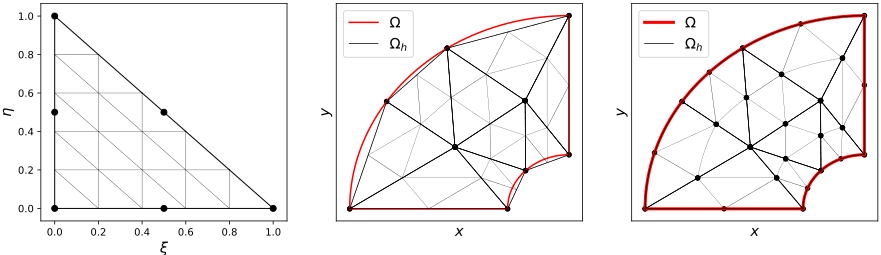
\includegraphics[width=1.\textwidth]{standart_quad_lin_example}
	\caption{Пример аппроксимации и разбиения области \(\Omega\) (<<линейные>> и <<квадратичные>> ячейки)}
	\label{pic:exampleapprox}
\end{figure}

В методе конечных элементов решение системы уравнений~(\ref{eq:generalPDE}) ищется в пространстве базисных функций, или функций формы, а не в физическом пространстве. Решение в каждой ячейке сетки представляется в виде линейной комбинации базисных функций \(\varphi_m(\mathbf x)\):
\begin{equation}\label{eq:Ureconstr}
\mathbf U(\mathbf x, t)\biggm|_{\mathbf{x} \in K_{ie}} = \sum\limits_{m=1}^{K_f} \mathbf u_m(t)\, \varphi_m(\mathbf x),
\end{equation}
где \(\mathbf u_m\) "--- коэффициенты этого разложения, которые являются основными неизвестными величинами в методе конечных элементов.

В данной работе в качестве базисных функций рассматриваются полиномы. Набор функций \(\varphi_m (\mathbf x),~m=\overline{1, K_f}\) образует базис в пространстве полиномов от трёх пространственных координат \((x, y, z)\) степени \(K\). В случае, когда решение уравнения~(\ref{eq:generalPDE}) непрерывно, использование мономов степени \(K\) является необходимым условием для достижения \((K+1)\)-го порядка точности "--- порядка сходимости численного решения при измельчении ячеек сетки. Количество базисных функций \(K_f\) связано с \(K\) соотношением:
\[
K_f = \frac{(K+1) (K+2) (K+3)}{6}.
\]

Существует несколько различных способов определения коэффициентов \(\mathbf u_m\). В методе Галёркина для этого каждое уравнение системы~(\ref{eq:generalPDE}) умножается на базисные функции и интегрируется по контрольному объёму \(\Theta\):
\begin{equation}\label{eq:intPDE}
\iiint\limits_{\Theta} \left(\frac{\partial\mathbf U}{\partial t} + \nabla\cdot \mathbf F\right) \varphi_m(\mathbf x)\: \mathrm d\mathbf x = \iiint\limits_{\Theta} \mathbf S\,\varphi_m(\mathbf x)\: \mathrm d\mathbf x,\quad m = \overline{1, K_f}.
\end{equation}
Подставив разложения~(\ref{eq:Ureconstr}) в соотношения~(\ref{eq:intPDE}) и расписав аппроксимации всех интегралов, получим систему из \(K_f\) уравнений для нахождения \(\mathbf u_m\).

В методе Галёркина с разрывными базисными функциями (РМГ, англ. \textenglish{DG~--- Discontinuous Galerkin}) в разных ячейках используются различные разложения вида (\ref{eq:Ureconstr}), поэтому на гранях ячеек зависимость \(\mathbf U(\mathbf x)\) является, вообще говоря, разрывной. В качестве \(\Theta\) в (\ref{eq:intPDE}) используется объём отдельной ячейки \(K_{ie}\). Таким образом, (\ref{eq:intPDE}) превращается в систему уравнений для нахождения коэффициентов \(\mathbf u_m\) в каждой ячейке. Для консервативности метода "--- выполнения глобальных законов сохранения "--- необходимо, чтобы потоки через общую грань двух соседних ячеек были одинаковы при записи уравнений баланса в каждой из этих ячеек. Так как разложения (\ref{eq:Ureconstr}) в соседних ячейках различны, то потоки через общую грань должны вычисляться по особой процедуре.

Вначале применим к уравнению (\ref{eq:intPDE}) преобразование:
\[
(\nabla\cdot \mathbf F)\, \varphi = \left(\nabla\cdot \mathbf F\,\varphi\right) - \mathbf F\,\nabla\varphi,
\]
а затем "--- формулу Остроградского--Гаусса. В результате получим систему уравнений:
\begin{multline*}
\iiint\limits_{K_{ie}} \frac{\partial \mathbf U}{\partial t} \varphi_m\: \mathrm d\mathbf x + \oint_{\Sigma_{ie}} \left(\mathbf F\cdot \mathbf n\right) \varphi_m\: \mathrm d\Sigma = \\
\iiint\limits_{K_{ie}} \left(\mathbf F\cdot \nabla\varphi_m\right) \mathrm d\mathbf x + \iiint\limits_{K_{ie}} \mathbf S\, \varphi_m\: \mathrm d\mathbf x,\quad m = \overline{1, K_f},
\end{multline*}
где \(K_{ie}\) "--- \(ie\)-я ячейка, \(\Sigma_{ie}\) "--- поверхность \(ie\)-й ячейки, \(\mathbf n\) "--- единичный вектор внешней нормали к элементу поверхности ячейки \(\mathrm d\Sigma\). Вводя следующие обозначения:
\[\begin{aligned}
\mathbf F_n &\equiv \left(\mathbf F\cdot \mathbf n\right) = \mathbf F_x n_x + \mathbf F_y n_y + \mathbf F_z n_z, \\
\mathbf F_m &\equiv \left(\mathbf F\cdot \nabla\varphi_m\right) = \mathbf F_x \frac{\partial \varphi_m}{\partial x} + \mathbf F_y \frac{\partial \varphi_m}{\partial y} + \mathbf F_z \frac{\partial \varphi_m}{\partial z},
\end{aligned}\]
получим более компактную запись:
\begin{multline}\label{eq:PDE:int:sep}
\iiint\limits_{K_{ie}} \frac{\partial \mathbf U}{\partial t} \varphi_m\: \mathrm d\mathbf x + \oint_{\Sigma_{ie}} \mathbf F_n \varphi_m\: \mathrm d\Sigma =\\
\iiint\limits_{K_{ie}} \mathbf F_m\: \mathrm d\mathbf x + \iiint\limits_{K_{ie}} \mathbf S\, \varphi_m\: \mathrm d\mathbf x,\quad m = \overline{1, K_f}.
\end{multline}

Коэффициенты разложения (\ref{eq:Ureconstr}) на известном временном слое обозначим через \(\mathbf u_m^n\), а на неизвестном временном слое "--- \(\mathbf u_m^{n+1}\). Приращения \(\Delta\mathbf u_m\) нужно найти из решения приближенного аналога системы уравнений (\ref{eq:PDE:int:sep}).

В случае, когда базисные функции ортонормированы, используя соотношения (\ref{eq:Ureconstr}), можно переписать систему (\ref{eq:PDE:int:sep}) в виде:
\begin{equation}\label{eq:ODE:dudt}
\frac{\mathrm d\mathbf u_m}{\mathrm d t} = \mathbf R_m,\quad m = \overline{1, K_f},
\end{equation}
где невязка \(\mathbf R_m\) включает интегралы по поверхности и объёму ячейки:
\begin{equation}\label{eq:R}
\mathbf R_m = -\oint_{\Sigma_{ie}} \mathbf F_n \varphi_m\: \mathrm d\Sigma + \iiint\limits_{K_{ie}} \mathbf F_m\: \mathrm d\mathbf x + \iiint\limits_{K_{ie}} \mathbf S\, \varphi_m\: \mathrm d\mathbf x,\quad m = \overline{1, K_f}.
\end{equation}

Таким образом, для нахождения коэффициентов разложения решения в каждой ячейке, необходимы способы вычисления объёмных и поверхностных интегралов.



%%================================
\section{Преобразования координат} \label{sect:transform}
%%================================

Элементы~\(K_{ie}\), на которые разбивается область~\(\Omega_h\), вообще говоря, могут быть произвольными. Однако вычисление интегралов по произвольным ячейкам "--- практически невыполнимая задача. Поэтому вводятся стандартные элементы, для которых известны методы получения точных значений интегралов от полиномов заданной степени. В качестве стандартных элементов используются симметричные фигуры, такие, как куб, квадрат, трёхмерный и двумерный симплексы. Эти элементы, в свою очередь, отображаются в физическое пространство, используя преобразования координат: линейные или квадратичные. Отображение из локального пространства элемента в физическое записывается в виде:
\begin{equation}\label{eq:gentransform}
\left\{\begin{array}{l}
x = x (\xi, \eta, \zeta), \\
y = y (\xi, \eta, \zeta), \\
z = z (\xi, \eta, \zeta), \\
\end{array}\right.\quad \xi, \eta, \zeta \in \hat \Omega.
\end{equation}
Для вычисления поверхностных интегралов по граням ячейки используется параметризация поверхности:
\begin{equation}\label{eq:genparam}
\left\{\begin{array}{l}
x = x (\xi, \eta), \\
y = y (\xi, \eta), \\
z = z (\xi, \eta), \\
\end{array}\right.\quad \xi, \eta \in \hat S.
\end{equation}

Преобразование~(\ref{eq:gentransform}) должно быть симметричным относительно переменных \(\xi\), \(\eta\) и \(\zeta\). При этом преобразования для каждой грани элемента не должны зависеть от координат остальных его вершин, чтобы соседние ячейки соприкасались по граням, т.\,е. чтобы не было <<нахлёстов>> элементов и <<дырок>> между ними.

В данной работе используются преобразования, которые могут быть записаны в следующем виде:
\begin{equation}\label{eq:transform3d}
\newcommand{\pat}[1]{{#1} = \sum_{i=1}^n {#1}_i N_i(\xi, \eta, \zeta)}
\left\{\begin{array}{l}
\pat{x}, \\
\pat{y}, \\
\pat{z}, \\
\end{array}\right.\quad \xi, \eta, \zeta \in \hat \Omega,
\end{equation}
\begin{equation}\label{eq:transform2d}
\newcommand{\pat}[1]{{#1} = \sum_{i=1}^m {#1}_i N_i(\xi, \eta)}
\left\{\begin{array}{l}
\pat{x}, \\
\pat{y}, \\
\pat{z}, \\
\end{array}\right.\quad \xi, \eta \in \hat S,
\end{equation}
где \((x_i, y_i, z_i)\) "--- координаты \(i\)-го узла в физическом пространстве, \(N_i\) "--- функция формы, равная единице в \(i\)-ом узле и нулю в других узлах стандартного элемента.

В работе рассматриваются два семейства конечных элементов: <<линейные>> и <<квадратичные>>. Тип элемента определяется количеством узловых точек на рёбрах. Так, в случае <<линейных>> элементов, количество узлов на каждом ребре ячейки равно двум. Для аппроксимации сложной геометрии небольшим количеством элементов простых <<линейных>> многогранников уже не достаточно. Возникает необходимость вводить <<квадратичные>> элементы, каждое ребро которых представлено тремя узловыми точками~(рис.~\ref{pic:exampleapprox}).

В следующих подразделах выписаны функции формы \(N_i\) для гексаэдров и тетраэдров, подробный вывод которых описан в~\cite{Zienkiewicz:2000:en}.



%%====================
\subsection{Гексаэдры}\label{subsect:hexatransform}
%%====================

\begin{figure}[h]
	{\centering
		\hfill
		\subbottom[Локальное пространство гексаэдра\label{pic:standarthexa}]{
			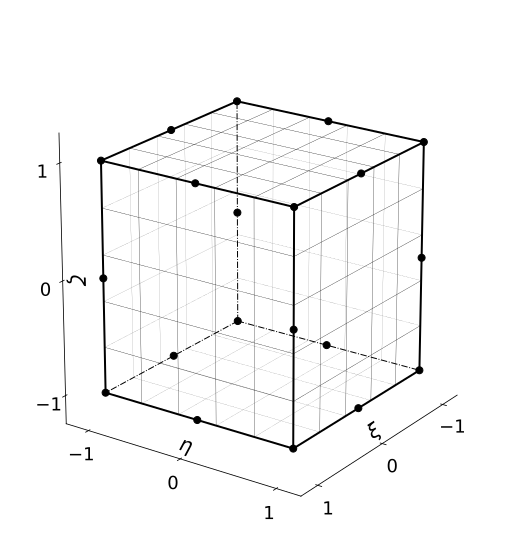
\includegraphics[width=0.48\textwidth]{standart_hexa}}
		\hfill
		\subbottom[Физическое пространство\label{pic:transformedhexa}]{
			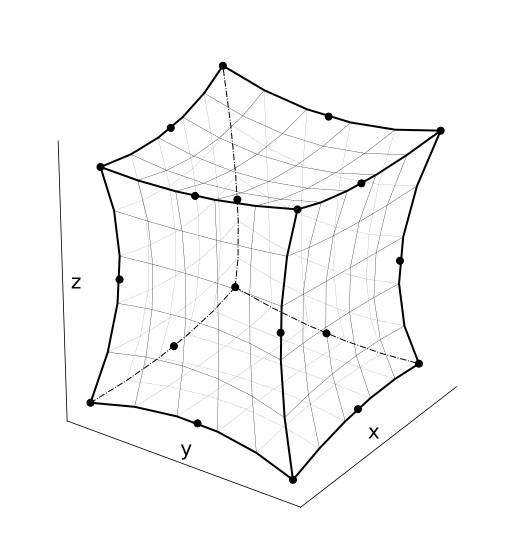
\includegraphics[width=0.48\textwidth]{transformed_hexa}}
		\hfill
	}
	\caption{Стандартный гексаэдр и его отображение в физическое пространство}
	\label{pic:hexatransform}
\end{figure}

Функции формы для <<линейных>> шестигранников имеют следующий вид:
\begin{equation}\label{eq:tr:hexa:lin}
N_i = \frac{1}{8} (1 + \xi_i \xi) (1 + \eta_i \eta) (1 + \zeta_i \zeta),
\end{equation}
где \((\xi_i, \eta_i, \zeta_i)\) "--- координаты i-й вершины <<стандартного>> шестигранника. В данной работе <<стандартный>> шестигранник представлен как куб с вершинами в точках \( \xi = \pm 1,\;\eta = \pm 1,\;\zeta = \pm 1\), как показано на рис. \ref{pic:standarthexa}.

На практике для представления <<квадратичных>> шестигранников часто используют так называемые <<серендиповы>> (serendipity) преобразования~\cite{Zienkiewicz:2000:en}. Они хороши тем, что используют информацию только о гранях ячейки вплоть до <<кубических элементов>>. Пример <<квадратичного>> гексаэдра в физическом пространстве показан на~рис.~\ref{pic:transformedhexa}. Функции формы <<квадратичных>> шестигранников имеют следующий вид:
\begin{itemize}
	\item для угловых узлов:
	\begin{multline}\label{eq:tr:hexa:quad}
	N_i = \frac{1}{8} (1 + \xi_i \xi) (1 + \eta_i \eta) (1 + \zeta_i \zeta)(\xi_i \xi + \eta_i \eta + \zeta_i \zeta - 2), \\
	\xi_i = \pm 1,\; \eta_i = \pm 1,\; \zeta_i = \pm 1,
	\end{multline}
	\item для серединных узлов:
	\begin{multline*}
	N_i = \frac{1}{4} (1 - \xi^2) (1 + \eta_i \eta) (1 + \zeta_i \zeta), \\
	\xi_i = 0,\; \eta_i = \pm 1,\; \zeta_i = \pm 1,\quad \text{и т.д.}
	\end{multline*}
\end{itemize}

Оценка степеней в преобразовании~(\ref{eq:transform3d}) приведена в~табл.~\ref{tab:transformorder:hexa}

\begin{table}[ht]
	\centering
	\caption{Степени полиномов в преобразовании (\ref{eq:transform3d}) для гексаэдров}
	\label{tab:transformorder:hexa}
	\smallskip
	\begin{tabular}{l l c c}
		\toprule
		элемент                           & степень             & преобразования & якобиана \\
		\midrule
		\multirow{2}{*}{<<линейный>>}     & суммарная           & 3              & 5 \\
		                                  & по одной переменной & 1              & 2 \\
		\midrule
		\multirow{2}{*}{<<квадратичный>>} & суммарная           & 4              & 9 \\
                                      & по одной переменной & 2              & 5 \\
		\bottomrule
	\end{tabular}
\end{table}



%%====================
\subsection{Тетраэдры}
%%====================

В отличие от шестигранников, у тетраэдров не все рёбра можно направить вдоль осей координат, что вызывает неудобство. Для компактной записи и для получения функций форм~(\ref{eq:transform3d}) и~(\ref{eq:transform2d}) удобно ввести барицентрические координаты \(L_1, L_2, L_3\) и \(L_4\). Они не являются независимыми и вводятся через систему линейных уравнений:
\begin{equation}\label{eq:barycentricsystem}
\left\{\begin{array}{l}
\xi   = L_1\xi_1   + L_2\xi_2   + L_3\xi_3   + L_4\xi_4,   \\
\eta  = L_1\eta_1  + L_2\eta_2  + L_3\eta_3  + L_4\eta_4,  \\
\zeta = L_1\zeta_1 + L_2\zeta_2 + L_3\zeta_3 + L_4\zeta_4, \\
1 = L_1 + L_2 + L_3 + L_4,
\end{array}\right.
\end{equation}
где \(\xi_i, \eta_i, \zeta_i\) "--- вершины стандартного тетраэдра.

\begin{figure}[h]
	{\centering
		\hfill
		\subbottom[треугольник]{
			\includegraphics[width=0.5\textwidth]{area_coordinates}}
		\hfill
		\subbottom[тетраэдр]{
			\includegraphics[width=0.4\textwidth]{volume_coordinates}}
		\hfill
	}
	\caption{Барицентрические координаты из~\cite{Zienkiewicz:2000:en}}
	\label{pic:barycentriccoord}
\end{figure}

В~\cite{Zienkiewicz:2000:en} проведен подробный анализ этих уравнений и было показано, что физический смысл барицентрических координат следующий~(рис.~\ref{pic:barycentriccoord}):
\begin{itemize}
	\item в двумерном случае это отношение площадей:
	\[L_1 = \frac{\text{площадь}\; P23}{\text{площадь}\; 123},\quad  \text{и т.д.,}\]
	\item в трёхмерном случае это отношение объёмов:
	\[L_1 = \frac{\text{объём}\; P234}{\text{объём}\; 1234},\quad \text{и т.д.}\]
\end{itemize}

Барицентрические координаты линейно меняются от единицы в соответствующем узле до нуля на противоположной грани. Тогда функции формы линейных элементов следующие~(рис.~\ref{pic:nodesorder:a}):
\begin{equation}\label{eq:tr:tetra:lin}
N_1 = L_1,\quad N_2 = L_2,\quad N_3 = L_3,\quad N_4 = L_4.
\end{equation}

\begin{figure}[t]
	{\centering
		\hfill
		\subbottom[<<линейные>>\label{pic:nodesorder:a}]{
			\includegraphics[width=0.45\textwidth]{tetra_4_nodes}}
		\hfill
		\subbottom[<<квадратичные>>\label{pic:nodesorder:b}]{
			\includegraphics[width=0.45\textwidth]{tetra_10_nodes}}
		\hfill
	}
	\caption{Семейства элементов и расположение узлов из~\cite{Zienkiewicz:2000:en}}
	\label{pic:nodesorder}
\end{figure}

Чтобы получить функции формы элементов более высокого порядка, можно воспользоваться интерполяционными полиномами Лагранжа. Для <<квадратичных>> элементов в~\cite{Zienkiewicz:2000:en} получены следующие функции формы:
\begin{itemize}
	\item для угловых узлов:
	\begin{equation}\label{eq:tr:tetra:quad}
	N_1 = (2L_1 - 1)L_1,\quad \text{и т.д.,}
	\end{equation}
	\item для серединных узлов:
	\[
	N_5 = 4L_1L_2, \quad \text{и т.д.}
	\]
\end{itemize}

В этой работе стандартным тетраэдром является стандартный трёхмерный симплекс: вершины расположены в точках \((0, 0, 0)\), \((1, 0, 0)\), \((0, 1, 0)\), \((0, 0, 1)\)~(рис.~\ref{pic:standartetra}). Тогда решение системы~(\ref{eq:barycentricsystem}) следующее:
\begin{equation}\label{eq:barycentriccoords}
\left\{\begin{array}{l}
L_1 = 1 - \xi - \eta - \zeta, \\
L_2 = \xi, \\
L_3 = \eta, \\
L_4 = \zeta. \\
\end{array}\right.
\end{equation}

Используя соотношения (\ref{eq:tr:tetra:lin}), (\ref{eq:tr:tetra:quad}) и (\ref{eq:barycentriccoords}), в табл.~\ref{tab:transformorder:tetra} получены оценки степени полиномов в преобразовании~(\ref{eq:transform3d}).

\begin{figure}[h]
	{\centering
		\hfill
		\subbottom[Локальное пространство тетраэдра\label{pic:standartetra}]{
			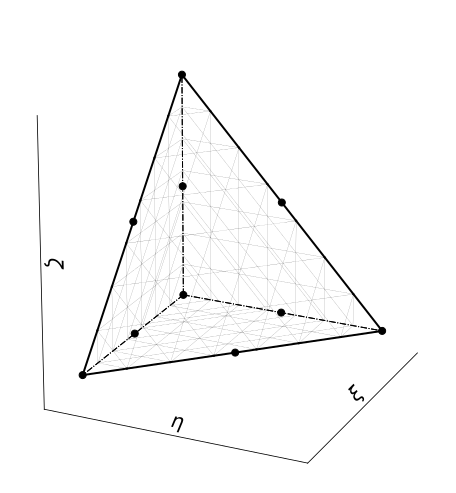
\includegraphics[width=0.48\textwidth]{standart_tetra}}
		\hfill
		\subbottom[Физическое пространство\label{pic:transformedtetra}]{
			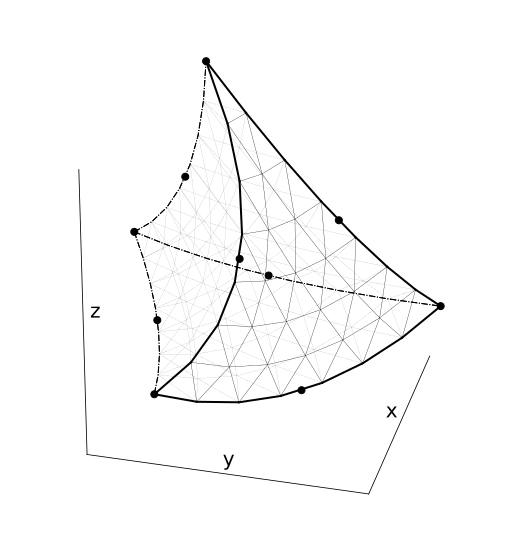
\includegraphics[width=0.48\textwidth]{transformed_tetra}}
		\hfill
	}
	\caption{Стандартный тетраэдр и его отображение в физическое пространство}
	\label{pic:tetratransform}
\end{figure}

\begin{table}[ht]
	\centering
	\caption{Степени полиномов в преобразовании (\ref{eq:transform3d}) для тетраэдров}
	\label{tab:transformorder:tetra}
	\smallskip
	\begin{tabular}{l l c c}
		\toprule
		элемент                           & степень             & преобразования & якобиана \\
		\midrule
		\multirow{2}{*}{<<линейный>>}     & суммарная           & 1              & 0 \\
		                                  & по одной переменной & 1              & 0 \\
		\midrule
		\multirow{2}{*}{<<квадратичный>>} & суммарная           & 2              & 3 \\
		                                  & по одной переменной & 2              & 3 \\
		\bottomrule
	\end{tabular}
\end{table}



%%================================
\subsection{Преобразование граней} \label{subsect:paramfaces}
%%================================

Чтобы провести вычисление поверхностного интеграла по одной из граней элемента~\(K_{ie}\), грань задается в параметрическом виде~(\ref{eq:transform2d})~(рис.~\ref{pic:parametricsurf}). Можно получить систему~(\ref{eq:transform2d}), которая параметрически задаёт конкретную грань, если добавить в~(\ref{eq:transform3d}) определяющее одну из граней соотношение:
\begin{itemize}
	\item в случае гексаэдров:
	\[\xi = \pm 1,\quad \eta = \pm 1,\quad \zeta = \pm 1,\]
	\item в случае тетраэдров:
	\[L_1 = 0,\quad L_2 = 0,\quad L_3 = 0,\quad L_4 = 0.\]
\end{itemize}

\begin{figure}[h]
	{\centering
		\hfill
		\subbottom[Локальное пространство\label{pic:parametricsurf:a}]{
			\includegraphics[width=0.4\textwidth]{parametric_surface_standart}}
		\hfill
		\subbottom[Физическое пространство\label{pic:parametricsurf:b}]{
			\includegraphics[width=0.5\textwidth]{parametric_surface_real}}
		\hfill
	}
	\caption{Пример параметрического задания грани}
	\label{pic:parametricsurf}
\end{figure}

Чтобы оценить степень подынтегрального выражения, необходимо определить степени полиномов в векторе
\begin{equation}\label{eq:normal}
\mathbf J(\xi, \eta) =
\begin{pmatrix}
\pfrac{x}{\xi} \\[1ex]
\pfrac{y}{\xi} \\[1ex]
\pfrac{z}{\xi} \\
\end{pmatrix}
\times
\begin{pmatrix}
\pfrac{x}{\eta} \\[1ex]
\pfrac{y}{\eta} \\[1ex]
\pfrac{z}{\eta} \\
\end{pmatrix}.
\end{equation}
Оценка степеней полиномов при параметрическом задании граней для гексаэдров приведена в~табл.~\ref{tab:paramorder:hexa}, а для тетраэдров в~табл.~\ref{tab:paramorder:tetra}, где за~\(\mathrm J_{x,y,z}(\xi, \eta)\) обозначен любой элемент вектора~\(\mathbf J\).

\begin{table}[h]
	\centering
	\caption{Степени полиномов при параметрическом задании граней (\ref{eq:transform2d}) гексаэдров}
	\label{tab:paramorder:hexa}
	\smallskip
	\begin{tabular}{l l c c}
		\toprule
		элемент                           & степень             & преобразования & \(\mathrm J_{x,y,z}(\xi, \eta)\) \\
		\midrule
		\multirow{2}{*}{<<линейный>>}     & суммарная           & 2              & 1 \\
		                                  & по одной переменной & 1              & 1 \\
		\midrule
		\multirow{2}{*}{<<квадратичный>>} & суммарная           & 3              & 4 \\
		                                  & по одной переменной & 2              & 3 \\
		\bottomrule
	\end{tabular}
\end{table}

\begin{table}[h]
	\centering
	\caption{Степени полиномов при параметрическом задании граней (\ref{eq:transform2d}) тетраэдров}
	\label{tab:paramorder:tetra}
	\smallskip
	\begin{tabular}{l l c c}
		\toprule
		элемент                           & степень             & преобразования & \(\mathrm J_{x,y,z}(\xi, \eta)\) \\
		\midrule
		\multirow{2}{*}{<<линейный>>}     & суммарная           & 1              & 0 \\
		                                  & по одной переменной & 1              & 0 \\
		\midrule
		\multirow{2}{*}{<<квадратичный>>} & суммарная           & 2              & 1 \\
		                                  & по одной переменной & 2              & 1 \\
		\bottomrule
	\end{tabular}
\end{table}



%%==============================
\section{Правила интегрирования}\label{sect:cubatures}
%%==============================

В методе Галёркина с разрывными базисными функциями один из шагов в алгоритме "--- это вычисление поверхностных и объёмных интегралов по ячейкам расчётной области:
\[
\begin{aligned}
\iiint\limits_{K_{ie}}&F(x, y, z)\: \mathrm d\mathbf x,\\
\iint\limits_{\Sigma_{ie}}&\mathbf F(x, y, z)\cdot \mathrm d\mathbf S,
\end{aligned}
\]
где \( K_{ie}\) "--- элементы, на которое было разбито исходное пространство~(см.~\ref{sect:DG}), \(\Sigma_{ie}\) "--- одна из граней \( K_{ie}\). Используя преобразование~(\ref{eq:gentransform}) и параметризацию для граней~(\ref{eq:genparam}), получим:
{
	\newcommand*{\vecxi}{\xi, \eta, \zeta}
	\begin{multline} \label{eq:volumeintegral}
	\iiint\limits_{K_{ie}}F(x, y, z)\: \mathrm d\mathbf x =\\
	\iiint\limits_{\hat\Omega}F\big(x(\vecxi), y(\vecxi), z(\vecxi)\big) \left|\det\mathbf J(\vecxi)\right|\:\mathrm d\xi\,\mathrm d\eta\, \mathrm d\zeta,
	\end{multline}
}
\begin{equation} \label{eq:surfaceintegral}
\iint\limits_{\Sigma_{ie}}\mathbf F(x, y, z)\cdot \mathrm d\mathbf{S} =
\iint\limits_{\hat{S}}\mathbf F(x(\xi, \eta), y(\xi, \eta), z(\xi, \eta))\cdot \mathbf J(\xi, \eta)\: \mathrm d\xi\, \mathrm d\eta,
\end{equation}
где \(\hat S\) "--- стандартный двумерный элемент, \(\mathbf J(\xi, \eta, \zeta)\) "--- матрица Якоби преобразования~(\ref{eq:transform3d}), \(\mathbf J(\xi, \eta)\) определен в~(\ref{eq:normal}).

На каждом элементе~\( K_{ie}\) вводятся базисные функции, на которые раскладывается искомое решение задачи. В данной работе в качестве базисных функций используют полиномы~(см.~раздел~\ref{sect:DG}). Поэтому подынтегральные функции "--- это полиномы некоторой степени.

Оценим степени подынтегральных выражений~(\ref{eq:volumeintegral}) и~(\ref{eq:surfaceintegral}). Обозначим за~\(k_F\) полную степень полинома~\(F\), за~\(k_T\) степень отображения, и за~\(k_J\) степень якобиана отображения. Получим, что
\begin{equation}\label{eq:intdegree}
k = k_F k_T + k_J.
\end{equation}

Для численного одномерного интегрирования используются квадратурные правила. \textit{Квадратурное правило} обычно определяется множеством различных точек \(\bigl\{x_0,\ldots, x_n \bigr\}\) в диапазоне \([-1,\, 1]\) и множеством соответствующих коэффициентов \(\bigl\{\alpha_0,\ldots, \alpha_n \bigr\}\), называемых весами, которые удовлетворяют соотношению:
\begin{equation}\label{eq:quadrule}
\int_{-1}^{1} p_k(x)\: \mathrm dx \; = \; \sum_{i = 0}^{n} \alpha_i p_k(x_i),
\end{equation}
где~\(p_k(x)\) "--- полином степени~\(k\). Порядок точности интегрирования определяется как максимальная степень~\(k\), для которой  выполнено~(\ref{eq:quadrule}).

Примечательно, что в некоторых квадратурных правилах изначально <<фиксируются>> квадратурные точки, что ведет к уменьшению максимально возможного порядка точности. Так, например, в методе трапеций изначально <<фиксируют>> точки \(x_0 = -1\), \(x_1 = 1\), а затем считают соответствующие веса: \(\alpha_0 = \alpha_1 = 1\). В результате метод является точным только для полиномов первой степени. В квадратурах Гаусса же точки не <<фиксируются>>. Как следствие, для того же количества точек получаем 3-й порядок точности. Снижение количества квадратурных точек позволяет ускорить работу численной схемы. Поэтому целесообразней использовать именно квадратуры Гаусса для одномерного интегрирования.

Стоит отметить, что квадратуры Гаусса можно вывести для любого порядка точности путём нахождения нулей полиномов Лежандра. Для~\(N\) точек максимальная степень подынтегрального полинома, для которого выполнено~(\ref{eq:quadrule}), равна \(2N - 1\).

В многомерном случае в определении~(\ref{eq:quadrule}) \(x\) заменяется на вектор~\(\mathbf x\), а область интегрирования на некоторый элемент, по которому необходимо проводить интегрирование. Элемент, вообще говоря, может быть произвольным. В данной работе рассматриваются два таких элемента "--- гексаэдр и тетраэдр.

Отмечу, что в методе Галёркина с разрывными базисными функциями подынтегральные выражения в объёмном интеграле "--- это полиномы степени \(k_F = 2K\), а в поверхностном "--- полиномы степени \(k_F = 2K + 1\), где \(K\) "--- это степень базисных функций, см. раздел~\ref{sect:DG} и~\cite{Podaruev:2017}.



%%====================
\subsection{Гексаэдры}
%%====================

В таблицах~\ref{tab:integrationorder:hexa} и~\ref{tab:integrationparam:hexa} приведены степени подынтегральных выражений в объёмном~(\ref{eq:volumeintegral}) и поверхностном~(\ref{eq:surfaceintegral}) интегралах.

\begin{table}[h]
	\centering
	\caption{Степени подынтегрального выражения в интеграле по объёму (\ref{eq:volumeintegral})}
	\label{tab:integrationorder:hexa}
	\smallskip
	\begin{tabular}{l l c}
		\toprule
		элемент                                    & степень             & \\
		\midrule
		\multirow{2}{*}{<<линейный>> гексаэдр}     & суммарная           & \(3k_F + 5\) \\
		                                           & по одной переменной & \( k_F + 2\) \\
		\midrule
		\multirow{2}{*}{<<квадратичный>> гексаэдр} & суммарная           & \(4k_F + 9\) \\
		                                           & по одной переменной & \(2k_F + 5\) \\
		\bottomrule
	\end{tabular}
\end{table}

\begin{table}[h]
	\centering
	\caption{Степени подынтегрального выражения в поверхностном интеграле (\ref{eq:surfaceintegral})}
	\label{tab:integrationparam:hexa}
	\smallskip
	\begin{tabular}{l l c}
		\toprule
		элемент                                            & степень             & \\
		\midrule
		\multirow{2}{*}{грань <<линейного>> гексаэдра}     & суммарная           & \(2k_F + 1\) \\
		                                                   & по одной переменной & \( k_F + 1\) \\
		\midrule
		\multirow{2}{*}{грань <<квадратичного>> гексаэдра} & суммарная           & \(3k_F + 4\) \\
		                                                   & по одной переменной & \(2k_F + 3\) \\
		\bottomrule
	\end{tabular}
\end{table}

В случае шестигранников и квадратов, квадратурные правила могут быть получены из одномерных квадратур Гаусса~\cite{Tesini:2008:en}. Область интегрирования "--- стандартный шестигранник: \(\hat\Omega = [-1,\, 1]^3\). Рассмотрим интегрирование функции \(Q_k = \sum_{i, j, h = 0}^k c_{ijh}\xi^i\eta^j\zeta^h\):
\[
\newcommand{\cubature}[3]{\sum_{#1=1}^{N} \alpha_#1 {#2}^#3_#1}
\begin{aligned}
\iiint\limits_{\hat\Omega} Q_k\: \mathrm d\Omega &=  \sum_{i, j, h = 0}^k c_{ijh} \int_{-1}^{1} \int_{-1}^{1} \int_{-1}^{1} \xi^i \eta^j \zeta^h \:d\xi\:d\eta\:d\zeta = \\
&=	\sum_{i, j, h = 0}^k c_{ijh} \int_{-1}^{1} \xi^i\: \mathrm d\xi \int_{-1}^{1} \eta^j\: \mathrm d\eta \int_{-1}^{1} \zeta^h\: \mathrm d\zeta = \\
&= \sum_{i, j, h = 0}^k c_{ijh} (\cubature{p}{\xi}{i})(\cubature{m}{\eta}{j})(\cubature{n}{\zeta}{h}) = \\
&= \sum_{p, m, n = 1}^N \alpha_p\alpha_m\alpha_n Q_k(\xi_p, \eta_m, \zeta_n),
\end{aligned}
\]
где \(N\) "--- количество квадратурных точек, необходимых для интегрирования полинома максимально \(k\)-й степени, \(\alpha_i\) "--- вес для соответствующей квадратурной точки~(\ref{eq:quadrule}). Таким образом, используя квадратуры Гаусса, можно получить правила интегрирования произвольной точности по кубу. В двумерном случае вывод аналогичный. Графическое изображение кубатурных точек в случае квадрата приведено на рис.~\ref{pic:cubature_rect}.

\begin{figure}[h]
	\centering
	\includegraphics[width=0.49\textwidth]{cubature_rule_6}
	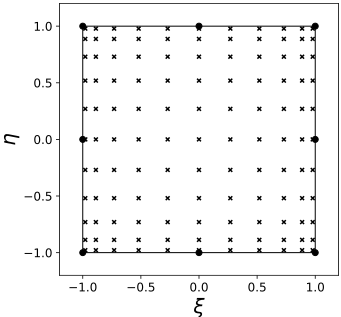
\includegraphics[width=0.49\textwidth]{cubature_rule_11}
	\caption{ Кубатурные точки для квадрата, \(N = 6\) и \(N = 11\)}
	\label{pic:cubature_rect}
\end{figure}

Посчитаем в случае куба для заданной степени \(\text{deg}_{\xi, \eta, \zeta}\) по \(\xi, \eta, \zeta\) количество точек \(N_{\text{cube}}\) и \(N_{\text{square}}\), необходимых для точного интегрирования полинома:
\[
\begin{aligned}
2&N-1 = \text{deg}_\xi\\
&N = \left\lceil \frac{\text{deg}_\xi + 1}{2} \right\rceil \\
&N_{\text{square}} = \left\lceil \frac{\text{deg}_{\xi, \eta} + 1}{2} \right\rceil^2 \\
&N_{\text{cube}} = \left\lceil \frac{\text{deg}_{\xi, \eta, \zeta} + 1}{2} \right\rceil^3
\end{aligned}
\]
Например, для интегрирования по кубу полиномов 9-й степени по \(\xi, \eta, \zeta\) (суммарная степень при этом может быть 27) получаем 125 точек.

Заметим, что, несмотря на высокие суммарные степени полиномов в подынтегральном выражении (см.~табл.~ \ref{tab:integrationorder:hexa} и~\ref{tab:integrationparam:hexa}), каждая переменная в них входит в значительно меньшей степени. Это позволяет снизить количество точек в квадратурных правилах, построенных как декартово произведение одномерных правил.


Рассмотрим теперь интегрирование по объёму и по поверхности одной из грани элемента~\(K_{ie}\):
{
\newcommand*{\vecxi}{\xi, \eta, \zeta}
\newcommand*{\vecxiind}[3]{\xi_#1, \eta_#2, \zeta_#3}
\begin{multline*}
	\iiint\limits_{K_{ie}}F(x, y, z)\: \mathrm d\mathbf x = \iiint\limits_{\hat\Omega}\hat F(\vecxi)\:\mathrm d\xi\,\mathrm d\eta\, \mathrm d\zeta, = \\
	\iiint\limits_{\hat\Omega}F\big(x(\vecxi), y(\vecxi), z(\vecxi)\big) \left|\det\mathbf J(\vecxi)\right|\:\mathrm d\xi\,\mathrm d\eta\, \mathrm d\zeta, = \\
	\sum_{p, m, n = 1}^N \alpha_p\alpha_m\alpha_n F\big(x(\vecxiind{p}{m}{n}), y(\vecxiind{p}{m}{n}), z(\vecxiind{p}{m}{n})\big) \left|\det\mathbf J(\vecxiind{p}{m}{n})\right|,
\end{multline*}
}
\begin{multline*}
\iint\limits_{\Sigma_{ie}}\mathbf F(x, y, z)\cdot \mathrm d\mathbf{S} =
\iint\limits_{\hat{S}}\mathbf F(x(\xi, \eta), y(\xi, \eta), z(\xi, \eta))\cdot \mathbf J(\xi, \eta)\: \mathrm d\xi\, \mathrm d\eta = \\
\sum_{p, m = 1}^M \alpha_p\alpha_m \mathbf F\big(x(s\xi_p, \eta_m), y(\xi_p, \eta_m), z(\xi_p, \eta_m)\big) \cdot \mathbf J(\xi_p, \eta_m),
\end{multline*}
где \(\alpha_i\) "--- вес для соответствующей квадратурной точки (\ref{eq:quadrule}), \(N, M\) "--- количество квадратурных точек в методе Гаусса.



%%====================
\subsection{Тетраэдры} \label{subsect:tetrarules}
%%====================

Используя соотношение~(\ref{eq:intdegree}) и результаты оценки степеней преобразования для тетраэдра из~табл.~\ref{tab:transformorder:tetra}, в таблицах~\ref{tab:integrationorder:tetra} и~\ref{tab:integrationparam:tetra} получены степени подынтегральных выражений в объёмном~(\ref{eq:volumeintegral}) и поверхностном~(\ref{eq:surfaceintegral}) интегралах.

\begin{table}[h]
	\centering
	\caption{Степени подынтегрального выражения в интеграле по объёму (\ref{eq:volumeintegral})}
	\label{tab:integrationorder:tetra}
	\smallskip
	\begin{tabular}{l l c}
		\toprule
		элемент                                    & \multicolumn{2}{l}{степень} \\
		\midrule
		\multirow{2}{*}{<<линейный>> тетраэдр}     & суммарная           & \(k_F\) \\
		                                           & по одной переменной & \(k_F\) \\
		\midrule
		\multirow{2}{*}{<<квадратичный>> тетраэдр} & суммарная           & \(2k_F + 3\) \\
		                                           & по одной переменной & \(2k_F + 3\) \\
		\bottomrule
	\end{tabular}
\end{table}

\begin{table}[h]
	\centering
	\caption{Степени подынтегрального выражения в поверхностном интеграле (\ref{eq:surfaceintegral})}
	\label{tab:integrationparam:tetra}
	\smallskip
	\begin{tabular}{l l c}
		\toprule
		элемент & \multicolumn{2}{l}{степень} \\
		\midrule
		\multirow{2}{*}{грань <<линейного>> тетраэдра}     & суммарная           & \(k_F\) \\
		                                                   & по одной переменной & \(k_F\) \\
		\midrule
		\multirow{2}{*}{грань <<квадратичного>> тетраэдра} & суммарная           & \(2k_F + 1\) \\
		                                                   & по одной переменной & \(2k_F + 1\) \\
		\bottomrule
	\end{tabular}
\end{table}

В случае тетраэдров и треугольников получение кубатурных правил сложнее. Можно, впрочем, используя кубатурные правила для гексаэдров, получить кубатурные правила для тетраэдров с помощью преобразования координат. В качестве примера получим кубатурные правила для треугольника. Воспользуемся уже полученными формулами для линейного преобразования гексаэдра~(\ref{eq:tr:hexa:lin}) (\(\zeta \equiv 1\)) и преобразуем квадрат в треугольник, совместив верхние вершины, как показано на~рис.~\ref{pic:cub:tri:first}:
\begin{equation}\label{eq:totri}
\left\{\begin{array}{l}
\xi = -\frac{1}{4} (\tilde{\xi}\tilde{\eta} + \tilde{\eta} - \tilde{\xi} - 1), \\
\eta = \frac{1}{2} (\tilde{\eta} + 1). \\
\end{array} \right.
\end{equation}
Якобиан отображения:
\[
\det\mathbf J =
\begin{vmatrix}
\frac{1}{4} (1 - \tilde{\eta}) & \frac{1}{4} (1 - \tilde{\xi}) \\
0 & \frac{1}{2}
\end{vmatrix} = \frac{1}{8} (1 - \tilde{\eta}).
\]

\begin{figure}[h]
	{\centering
		\hfill
		\subbottom[Исходный квадрат\label{pic:cub:tri:first:init}]{
			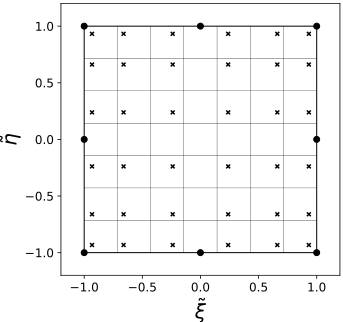
\includegraphics[width=0.48\textwidth]{rect_to_tri_before}}
		\hfill
		\subbottom[Полученный треугольник\label{pic:cub:tri:first:transformed}]{
			\includegraphics[width=0.48\textwidth]{rect_to_tri_after}}
		\hfill
	}
	\caption{Один из способов получения кубатурных правил}
	\label{pic:cub:tri:first}
\end{figure}

\begin{figure}[h]
	{\centering
		\hfill
		\subbottom[Неоптимальное кубатурное правило, \(N = 16\)]{
			\includegraphics[width=0.48\textwidth]{6_tri_not_opti}}
		\hfill
		\subbottom[Оптимизированное кубатурное правило, \(N = 12\)]{
			\includegraphics[width=0.48\textwidth]{6_tri_opti}}
		\hfill
	}
	\caption{Сравнение кубатурных правил 6-го порядка для треугольника}
	\label{pic:cub:comparasion}
\end{figure}

Из рис.~\ref{pic:cub:tri:first:transformed} видно, что кубатурные точки получились несимметричными, а также имеется сильное сгущение точек в верхней части треугольника. В численных расчётах это не очень хорошо: мы <<получаем>> много информации из одной части элемента и намного меньше из других. Количество кубатурных точек получилось неоптимальным. Существуют уже готовые симметричные кубатурные правила для тетраэдров и треугольников. Более того, если существующие кубатурные правила не подходят, можно воспользоваться алгоритмом поиска кубатурных правил, см.~\cite{SukumarCubatureRules:2020:en}. Для реализации интегрирования по тетраэдрам в программе~\cite{VolkovA:2010:ru} были использованы уже готовые оптимизированные симметричные кубатурные правила~\cite{CubatureRules}. На рис.~\ref{pic:cub:comparasion} приведены сравнения оптимизированных правил и правил, полученных с использованием (\ref{eq:totri}) для интегрирования по треугольнику полиномов \(\mathbf P (\xi, \eta)\) суммарной степени 6. Видно, что количество кубатурных точек меньше в случае оптимизированных правил.           % Глава 1
% !TEX encoding   = UTF8
% !TEX spellcheck = ru_RU

%%=================================
\chapter{Реализация и тестирование}
%%=================================

%%==========================================
\section{Особенности программной реализации}
%%==========================================

Структура кода расчётного модуля ZOOM DG выстроена таким образом, что для внедрения поддержки тетраэдральных элементов достаточно добавить правила преобразования и правила интегрирования. Идеи в коде представлены в виде типов. Так, например, идея кубатурных правил в коде выражена в виде типов \code{QRSide} и \code{QRCell}. А преобразование элементов представлено типами \code{ShapeFunctionSet2D} и \code{ShapeFunctionSet3D}. В виду существенных различий в вычислениях, связанных с объёмом, и в вычислениях, связанных с поверхностями, выделяются 2 иерархии классов: одна "--- для поверхностей, другая "--- для объёмов.



%%=========================
\subsection{Преобразования элементов} \label{subsect:2part:transform}
%%=========================

\begin{figure}[h]
	\centering
	\begin{tikzpicture}[nodes={font=\ttfamily\small, draw},
	rounded corners, level distance=10ex, >=Stealth]
	\graph [layered layout, components go right top aligned, edge=<-]
	{
		ShapeFunctionSet2D -> {
			QuadLinearElement[as=\tcol{QuadLinear\\Element}],
			QuadQuadraticElement[as=\tcol{QuadQuadratic\\Element}]
		};
		ShapeFunctionSet2D ->[blue] {
			TriLinearElement[blue, as=\tcol{TriLinear\\Element}],
			TriQuadraticElement[blue, as=\tcol{TriQuadratic\\Element}]
		};
	};
	\begin{scope}[on background layer]
	\node [draw, rounded corners,
	fit=(ShapeFunctionSet2D) (QuadLinearElement) (TriQuadraticElement)] {};
	\end{scope}
	\end{tikzpicture}
	\caption{Иерархия классов, реализующих преобразования граней}
	\label{pic:shapefunctions2d}
\end{figure}

\begin{figure}[h]
	\centering
	\begin{tikzpicture}[nodes={font=\ttfamily\small, draw},
	rounded corners, level distance=10ex, >=Stealth]
	\graph [layered layout, components go right top aligned, edge=<-]
	{
		ShapeFunctionSet3D -> {
			HexaLinearElement[as=\tcol{HexaLinear\\Element}],
			HexaQuadraticElement[as=\tcol{HexaQuadratic\\Element}]
		};
		ShapeFunctionSet3D ->[blue] {
			TetraLinearElement[blue, as=\tcol{TetraLinear\\Element}],
			TetraQuadraticElement[blue, as=\tcol{TetraQuadratic\\Element}]
		};
	};
	\begin{scope}[on background layer]
	\node [draw, rounded corners,
	fit=(ShapeFunctionSet3D) (HexaLinearElement) (TetraQuadraticElement)] {};
	\end{scope}
	\end{tikzpicture}
	\caption{Иерархия классов, реализующих преобразования элементов}
	\label{pic:shapefunctions3d}
\end{figure}

Ниже приведены фрагменты объявления базового класса преобразования поверхностных элементов~\ref{pic:shapefunctions2d}:

\begin{minted}[fontsize=\footnotesize, linenos]{C++}
class ShapeFunctionSet2D
{
protected:
  using ShapeFunc = std::function<QReal (QReal,QReal)>;

  vector<ShapeFunc> F;
  vector<ShapeFunc> dF_dXi, dF_dEta;

public:
  // ...

  zVec<QReal> transform (const vector<zVec<QReal>> &Xn,
                         QReal xi, QReal eta,
                         zVec<QReal> &N) const;
};
\end{minted}

\noindent
и фрагменты объявления базового класса преобразования объёмных элементов~\ref{pic:shapefunctions3d}:

\begin{minted}[fontsize=\footnotesize, linenos]{C++}
class ShapeFunctionSet3D
{
protected:
  using ShapeFunc = std::function<QReal (QReal,QReal,QReal)>;

  vector<ShapeFunc> F;
  vector<ShapeFunc> dF_dXi, dF_dEta, dF_dZeta;

public:
  // ...

  zVec<QReal> transform (const vector<zVec<QReal>> &Xn,
                         QReal xi, QReal eta, QReal zeta,
                         QReal &J) const;
};
\end{minted}

Базовые классы хранят набор функций формы и их производных и предоставляют метод \code{transform}, выполняющий преобразование в соответствии с соотношением~(\ref{eq:transform3d}) в трёхмерном случае и в соответствии с~(\ref{eq:transform2d}) в двумерном. Попутно производится вычисление элемента поверхности~\code{N} согласно формуле~(\ref{eq:normal}) и якобиана преобразования~\code{J}.

Конкретные наборы функций формы задаются при помощи производных классов. Например, ниже приведено объявление класса для задания <<линейного>> элемента поверхности тетраэдра:
\begin{minted}[fontsize=\footnotesize, linenos]{C++}
TriLinearElement::TriLinearElement ()
{
  // shape functions for corner nodes
  F.push_back ([](QReal xi, QReal eta) {return 1. - eta - xi;});
  F.push_back ([](QReal xi, QReal    ) {return xi;});
  F.push_back ([](QReal   , QReal eta) {return eta;});


  // derivative of shape functions with respect to xi
  dF_dXi.push_back ([](QReal, QReal) {return -1.;});
  dF_dXi.push_back ([](QReal, QReal) {return  1.;});
  dF_dXi.push_back ([](QReal, QReal) {return  0.;});


  // derivative of shape functions with respect to eta
  dF_dEta.push_back ([](QReal, QReal) {return -1.;});
  dF_dEta.push_back ([](QReal, QReal) {return  0.;});
  dF_dEta.push_back ([](QReal, QReal) {return  1.;});


  assert ( F      .size() == 3);
  assert (dF_dXi  .size() == 3);
  assert (dF_dEta .size() == 3);
}
\end{minted}

Функции формы и их производные располагаются в соответствующем векторе согласно нумерации узлов преобразования. В программе принята такая же нумерация, как и в Gmsh~\cite{Gmsh}. Таким образом, для преобразования тетраэдральных элементов необходимо было реализовать четыре класса, используя формулы (\ref{eq:tr:tetra:lin}) и (\ref{eq:tr:tetra:quad}). Двумерные преобразования получаются из трёхмерных, если добавить к ним дополнительное соотношение~(см.~подраздел~\ref{subsect:paramfaces}). Формулы для <<квадратичного>> элемента получаются довольно громоздкими, в них легко ошибиться. Был написан скрипт на \code{Python}~\cite{Python} с использованием библиотеки символьной математики \code{SymPy}~\cite{SymPy}, генерирующий фрагменты кода. Такой подход позволяет автоматизировать процесс и избавляет программиста от рутины, которая часто приводит к ошибкам.



%%=================================
\subsection{Правила интегрирования}
%%=================================

\begin{figure}[h]
	\centering
	\begin{tikzpicture}[nodes={font=\ttfamily\small, draw},
	                    rounded corners, level distance=5ex, >=Stealth]
	\graph [layered layout, components go right top aligned, edge=<-]
	{
		QRCell -> QRHexa -> {
			QRHexaOptimized,
			QRHexaGaLe
		};
		QRCell ->[blue] QRTetra[blue, text=blue]
		       ->[blue] QRTetraOptimized[blue, text=blue]
		       ->[blue] {
			QRTetraFirst[blue, as={QRTetra\_1\_1}],
			QRTetraJth[blue, as={...}],
			QRTetraNth[blue, as={QRTetra\_8\_43}]
		};
		QRTetra ->[blue, dashed] QRTetraGaLe[blue, dashed, text=blue, edge=dashed];
	};

	\begin{scope}[on background layer]
		\node [draw, rounded corners,
		       fit=(QRCell) (QRHexaOptimized) (QRTetraGaLe) (QRTetraNth)] {};
	\end{scope}
	\end{tikzpicture}
	\caption{Иерархия классов кубатурных правил интегрирования по объёму}
	\label{pic:cell:integrationrules}
\end{figure}

\begin{figure}[h]
	\centering
	\begin{tikzpicture}[nodes={font=\ttfamily\small, draw},
	                    rounded corners, level distance=5ex, >=Stealth]
	\graph [layered layout, components go right top aligned, edge=<-]
	{
		QRSide -> QRQuad -> {
			QRQuadOptimized,
			QRQuadGaLe
		};
		QRSide ->[blue] QRTri[blue, text=blue]
		       ->[blue] QRTriOptimized[blue, text=blue]
		       ->[blue] {
			QRTriFirst[blue, as={QRTri\_1\_1}],
			QRTriJth[blue, as={...}],
			QRTriNth[blue, as={QRTri\_13\_37}]
		};
		QRTri ->[blue, dashed] QRTriGaLe[blue, dashed, text=blue, edge=dashed];
	};

	\begin{scope}[on background layer]
	\node [draw, rounded corners,
	       fit=(QRSide) (QRQuadOptimized) (QRTriGaLe) (QRTriNth)] {};
	\end{scope}
	\end{tikzpicture}
	\caption{Иерархия классов кубатурных правил интегрирования по поверхности}
	\label{pic:side:integrationrules}
\end{figure}

Реализации двумерных и трёхмерных правил очень похожи, поэтому рассмотрим только двумерный случай. Базовый класс \code{QRSide} хранит координаты и веса квадратурных точек, а также для справочных целей максимальный порядок полинома, для которого формула абсолютно точна, и некий условный тип, несущий дополнительную информацию о квадратурном правиле (оптимальное, получено на основе одномерных квадратур Гаусса--Лежандра и т.\,п.). Интерфейс класса предоставляет небольшой набор методов, необходимых для работы: \code{size} "--- количество точек в формуле, \code{operator[]} "--- даёт доступ к координатам \code{i}-ой точки, \code{operator<} "--- определяет критерий упорядоченности (по увеличению вычислительной сложности, то есть количеству точек) правил во внешнем хранилище, и, наконец, методы \code{begin} и \code{end} обеспечивают поддержку конструкции языка \code{C++} <<\code{for-range}>>~\cite{Stroustrup:2013:en}. \code{is\_valid} "--- функция, проверяющая корректность кубатурной формулы, используя то свойство, что сумма всех кубатурных весов должна равняться объёму элемента. Так как у каждого элемента свой объём, эта функция является чисто виртуальной. Фрагменты класса приведены ниже:

\begin{minted}[fontsize=\footnotesize, linenos]{C++}
class QRSide : public z::Metadata
{
public:
  struct Point
  {
    QReal xi, eta;
    QReal weight;

    Point (QReal qxi, QReal qeta, QReal qweight)
      : xi {qxi}, eta {qeta}, weight {qweight}
    {}
  };

protected:
  std::vector<Point> points;

  virtual bool is_valid (size_t npoints, QReal eps) const = 0;

  // ...

public:
  const size_t order;
  const QRType type {QRType::Unknown};

  const Point & operator [] (size_t i) const;

  bool operator < (const QRSide& rhs) const;

  size_t size () const  {return points.size();}

  std::vector<Point>::const_iterator begin () const;
  std::vector<Point>::const_iterator end   () const;
};
\end{minted}

\noindent
Объявление класса \code{QRTetra} выглядит следующим образом:

\begin{minted}[fontsize=\footnotesize, linenos]{C++}
class QRTetra : public QRCell
{
protected:
  using QRCell::QRCell;  // inherits constructors

  bool is_valid (size_t npoints, QReal eps) const override;

public:
  ~QRTetra () override = 0;
};
\end{minted}

В данной работе использовались оптимизированные симметричные кубатурные правила~\cite{CubatureRules}, позволяющие интегрировать полиномы по тетраэдрам до 8-й степени и по треугольникам до 13-й степени. Под \textit{симметричными кубатурными правилами} (Fully Symmetric) подразумевается следующее: если кубатурное правило содержит точку \(\{L_1, L_2, L_3, L_4\}\) с весом~\(\alpha\), то оно также содержит и точку \(\{L_{p_1}, L_{p_2}, L_{p_3}, L_{p_4}\}\) с весом~\(\alpha\), где \(\{p_1, p_2, p_3, p_4\}\) "--- любая перестановка \(\{1, 2, 3, 4\}\). Если все \(L_i\) различны, то мы получим \(4! = 24\) кубатурных точек. В дальнейшем возможно добавление кубатурных правил произвольного порядка на основе квадратур Гаусса, см.~подраздел~\ref{subsect:tetrarules}.

Все оптимизированные квадратурные правила наследуют от класса \code{QRTriOptimized}:

\begin{minted}[fontsize=\footnotesize, linenos]{C++}
class QRTriOptimized : public QRTri
{
protected:
  void addFullySymmetric (QReal a, QReal b, QReal w);

  QRTriOptimized (size_t maxorder, QRType qrtype = QRType::Optimized)
    : QRTri {maxorder, qrtype}
  {}

public:
  ~QRTriOptimized () override = 0;
};
\end{minted}

Сложность реализации этого класса в трёхмерном случае заключалась в написании функции \code{addFullySymmetric}: требовалось рассмотреть 15 вариантов расположения кубатурной точки в тетраэдре, в последнем из которых необходимо было добавить 24 кубатурные точки. Для реализации функции, используя язык \code{Python}, был осуществлен перебор всех возможных вариантов и написан генератор исходного текста.

Ниже приведён пример класса, который реализует конкретную квадратурную формулу, состоящую из 4-х точек и точную для полиномов степени не выше 3-й:

\begin{minted}[fontsize=\footnotesize, linenos]{C++}
class QRTri_3_4 : public QRTriOptimized
{
public:
  QRTri_3_4 ();
};
\end{minted}

Как и в случае реализации правил преобразования элементов (см. подраздел~\ref{subsect:2part:transform}), основную работу по заполнению массива точек выполняет конструктор класса:

\begin{minted}[fontsize=\footnotesize, linenos]{C++}
QRTri_3_4::QRTri_3_4 ()
  : QRTriOptimized {3}
{
  QReal a = 0., b = 0., w = 0.;

  a = 0.333333333333333333333333333333333L;
  b = 0.333333333333333333333333333333333L;
  w = -0.28125L;
  addFullySymmetric (a, b, w);

  a = 0.2L;
  b = 0.2L;
  w = 0.260416666666666666666666666666666L;
  addFullySymmetric (a, b, w);

  assert (is_valid (4));
}
\end{minted}



%%====================
\section{Тестирование}
%%====================

%%===========================================
\subsection{Математическая постановка задачи}
%%===========================================

В качестве тестовой задачи рассматривается обтекание цилиндра невязким сжимаемым дозвуковым потоком. Характерная картина течения представлена на рис.~\ref{pic:result:mach}.

\begin{figure}[ht]
	\centering
	\includegraphics[width=1.\textwidth]{cylinder_tetra_fine_K3_Mach}
	\caption{Характерная картина течения при обтекании цилиндра. Показаны поле числа Маха, расчётная сетка и линии тока}
	\label{pic:result:mach}
\end{figure}

Обтекание цилиндра выбрано по следующим причинам: задача простая, а решение задачи экспериментально и теоретически изучено, см.~\cite{CylynderFlow:1994:en}. Обтекаемое тело имеет криволинейную форму, что позволяет протестировать преобразования координат и выяснить, как они влияют на ошибку в решении. Для выполнения расчёта необходимо построить расчётную сетку, а также задать начальные и граничные условия.

Сперва для знакомства с программой была построена расчётная сетка, состоящая из гексаэдральных элементов. Затем для тестирования была построена сетка из тетраэдральных элементов. Сетка строилась с использованием трёхмерного генератора конечно-элементных сеток Gmsh~\cite{Gmsh}.

Характеристики расчётной области: высота цилиндра равна 100 м, радиус цилиндра 1 м, внешняя граница расчётной области удалена от центра цилиндра на 1000 м. Для уменьшения флуктуаций вдоль оси цилиндра использовалась всего одна ячейка. Характеристический размер вдоль азимута равномерный, вдоль радиуса "--- подчиняется геометрической прогрессии.

\begin{figure}[h]
	\centering
	\includegraphics[width=0.8\textwidth]{hexa_mesh}
	\caption{Гексаэдральная расчётная сетка}
	\label{pic:hexamesh}
\end{figure}

\begin{figure}[h]
	\centering
	\includegraphics[width=0.8\textwidth]{tetra_mesh}
	\caption{Тетраэдральная расчётная сетка}
	\label{pic:tetramesh}
\end{figure}

Так как задача стационарная, а решение симметрично в верхней и нижней полуплоскостях, то сетка строилась только для половины расчётной области цилиндра. В плоскости симметрии используются симметричные граничные условия, на поверхности цилиндра твёрдая стенка без прилипания, а на внешней границе области "--- условие свободного вытекания.

В качестве начального условия было задано равномерное поле с параметрами, как в набегающем потоке: давление \(p_\infty = 100\,000\) Па, плотность \(\rho_\infty = 1.19\) кг/\(\text{м}^3\), скорость, направленная поперёк цилиндра, \(u_\infty = 50\) м/с, остальные компоненты скорости равны нулю.

Пример гексаэдральной и тетраэдральной расчётных сеток показан на рис.~\ref{pic:hexamesh} и рис.~\ref{pic:tetramesh}.



%%==================================
\subsection{Результаты тестирования}
%%==================================

Расчёты проводились с различными степенями базисных полиномов \(K~=~0, 1, 2, 3, 4\) для двух видов сеток: с <<линейными>> и <<квадратичными>> элементами. Характеристики расчётной сетки в обоих случаях одинаковы (см.~рис.~\ref{pic:tetramesh}): количество ячеек у цилиндра равно 3, коэффициент прогрессии равен 2. Сетка получилась довольно грубой: количество тетраэдров равно 315.

Известно, что сопротивление цилиндра в случае невязкого обтекания равно нулю, а поле полного давления равномерно во всем пространстве. По этим параметрам можно оценить ошибку.

\begin{figure}[ht]
	\centering
	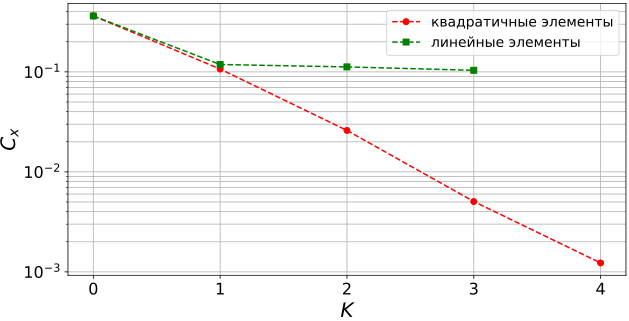
\includegraphics[width=0.8\textwidth]{Cx}
	\caption{Убывание ошибки в определении коэффициента сопротивления \(C_{x}\) в зависимости от порядка базисных функций \(K\)}
	\label{pic:Cx}
\end{figure}

На рис.~\ref{pic:Cx} показано убывание логарифма ошибки определения коэффициента сопротивления в зависимости от порядка базисных функций. Видно, что для \(K = 0\) и \(K = 1\) ошибки у <<квадратичных>> и <<линейных>> тетраэдров идентичны. Но с дальнейшим увеличением \(K\) ошибка в случае <<линейных>> элементов практически не убывает. Для расчёта на сетке с <<линейными>> элементами с \(K = 3\) пришлось сильно уменьшить шаг по времени, иначе метод не сходился. Из графика видно, что использование <<квадратичных>> элементов при \(K \geq 2\) позволяет уменьшить ошибку при вычислении сопротивления цилиндра на несколько порядков.

\begin{figure}[ht]
	\centering
	\includegraphics[width=0.7\textwidth]{K2_quad}
	\caption{Поле полного давления, \(K = 2\), <<квадратичные>> тетраэдры. Нечёткость картины связана с грубой визуализацией}
	\label{pic:p_stagnation}
\end{figure}

Рассмотрим теперь картину полного давления для разных порядков базисных функций \(K\). Полное давление вычисляется по следующей формуле: 
\[p_{0\infty} = p_\infty \left(1 + \frac{\gamma-1}{2}M_{\infty}^2\right)^\frac{\gamma}{\gamma - 1},\] 
где \(\gamma\) "--- показатель адиабаты, \(M\) "--- число Маха. Из рис.~\ref{pic:p_stagnation} видно, что за цилиндром возникает область падения поля полного давления. Рассмотрим точку \(\mathbf x_b\), расположенную сразу за цилиндром: \(x_b = 1\) м, \(y_b = 0\) м. Можно попытаться определить ошибку, вычислив \(\left|\Delta p_0\right| = \left|p_{0\infty} - p_0(\mathbf x_b)\right|\). На рис.~\ref{pic:p_error} показано убывание ошибки в зависимости от степени базисных функций в точке~\(\mathbf x_b\). Картина аналогична тому, что мы видели на рис.~\ref{pic:Cx}: при \(K = 0\) и \(K = 1\) ошибки идентичны, а при увеличении порядка~\(K\) ошибка в случае <<квадратичных>> элементов уменьшается больше, чем в случае <<линейных>>.

\begin{figure}[ht]
	\centering
	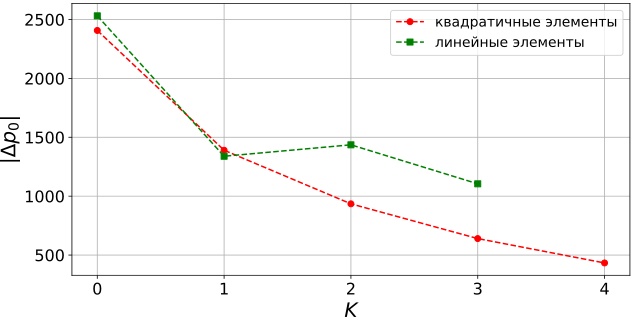
\includegraphics[width=0.8\textwidth]{p0}
	\caption{Убывание ошибки полного давления \(p_{0}\) в точке за цилиндром в зависимости от порядка базисных функций \(K\)}
	\label{pic:p_error}
\end{figure}

На рис.~\ref{pic:result:mach} показан результат единичного расчёта на подробной сетке. Количество рёбер у цилиндра равно 32, коэффициент геометрической прогрессии равен~\(1.075\). В качестве базисных функций были взяты полиномы 3 степени. К завершению расчёта в задаче прошло 50 секунд физического времени. Вычисления длились почти 5 суток на Core i7 Haswell. Общее количество тетраэдров составило 26436.           % Глава 2
%\include{dissertation/part3}           % Глава 3
% !TEX encoding   = UTF8
% !TEX spellcheck = ru_RU

%%==================
\Chapter{Заключение}
%%==================

%% Согласно ГОСТ Р 7.0.11-2011:
%% 5.3.3 В заключении диссертации излагают итоги выполненного исследования, рекомендации, перспективы дальнейшей разработки темы.
%% 9.2.3 В заключении автореферата диссертации излагают итоги данного исследования, рекомендации и перспективы дальнейшей разработки темы.
%% Поэтому имеет смысл сделать эту часть общей и загрузить из одного файла в автореферат и в диссертацию:

Основным результатом работы является внедрение поддержки тетраэдральных элементов в расчётный модуль ZOOM DG.

В ходе работы изучены правила преобразований координат для тетраэдров и гексаэдров, а также правила интегрирования по ним. Работа численного метода проверена на примере задачи дозвукового обтекания цилиндра. Результаты тестирования на грубой сетке показывают, что криволинейные элементы приводят к более точному описанию решения, а увеличение максимальной степени полиномов базисных функций на единицу "--- к уменьшению ошибки в определении коэффициента сопротивления цилиндра примерно на порядок.

В продолжение работы необходимо выполнить исследование сеточной сходимости и оценить порядок аппроксимации схем. Добавить вывод полей с подсеточным разрешением. И перейти к реализации поддержки других элементов: призм и пирамид.
      % Заключение
%\include{dissertation/acronyms}        % Список сокращений и условных обозначений
\include{dissertation/references}      % Список литературы

%%% Настройки для приложений
\appendix
% Оформление заголовков приложений ближе к ГОСТ:
\setlength{\midchapskip}{20pt}
\renewcommand*{\afterchapternum}{\par\nobreak\vskip \midchapskip}
\renewcommand\thechapter{\Asbuk{chapter}} % Чтобы приложения русскими буквами нумеровались

\include{dissertation/appendix}        % Приложения

\end{document}
